\section{Introduction}

Recapping, this thesis characterises an open innovation partnership as a temporary knowledge network. We can use social network analysis to evaluate knowledge sharing practices in open innovation partnerships. The last chapter argued human agency lies at the heart of tacit knowledge sharing and suggested autonomous motivation, the disposition to trust, and power-relations in various social contexts influence an individual's decision to share or seek out tacit knowledge. Table \ref{tab:propos} lists the seven propositions developed in Chapters 2 and 3 and how these relate to the four research questions stated in Chapter 1. The propositions serve as an analytical framework for mixed-method inquiry, not as testable hypotheses. \medskip

This chapter explains the methodology used to assess the propositions across three open innovation partnerships. It includes justifications for embracing a critical realist worldview and employing a case-based mixed-method research design. The chapter details the quantitative and qualitative procedures used to collect and analyse data and the critical realist process used to interpret the data. 

\begin{sidewaystable}[p]
\centering
\caption[Sub-research questions and related propositions]{Sub-research questions and related propositions.}
\label{tab:propos}
\renewcommand{\arraystretch}{1.2}
\resizebox{0.9\textwidth}{!}{%	
\begin{tabular}{lcl}
\toprule
 \multicolumn{1}{c}{Sub-research question} &&  \multicolumn{1}{c}{Related proposition(s)} \\ \midrule
 
\begin{minipage}{0.35\linewidth}\renewcommand{\theenumi}{\arabic{enumi}} \begin{enumerate} \setcounter{enumi}{0} \item What does the structure of tacit knowledge networks reveal about knowledge enacted in practice? \end{enumerate}\end{minipage} && \begin{minipage}{0.55\linewidth} \renewcommand{\theenumi}{\alph{enumi}} \begin{enumerate}
    \item Open innovation is about connecting practitioners across organisational and disciplinary boundaries so that they can apply their know-how in novel ways.
    \item Relative differences in absorptive capacity limit the potential value of inter-organisational knowledge networks. Reducing the cognitive distance between open innovation partners requires significant social interaction to support learning and the application of knowledge in practice.
\end{enumerate} \end{minipage} \\ \midrule
 
\begin{minipage}{0.35\linewidth}\renewcommand{\theenumi}{\arabic{enumi}} \begin{enumerate} \setcounter{enumi}{1} \item Does brokerage differ according to the type of knowledge being exchanged? \end{enumerate}\end{minipage} && \begin{minipage}{0.55\linewidth} \renewcommand{\theenumi}{\alph{enumi}} \begin{enumerate} \item Successful open innovation requires a combination of skilled brokerage and network closure. \end{enumerate} \end{minipage} \\ \midrule

\begin{minipage}{0.35\linewidth}\renewcommand{\theenumi}{\arabic{enumi}} \begin{enumerate} \setcounter{enumi}{2} \item To what extent does self-determination drive tacit knowledge sharing in open innovation? \end{enumerate} \end{minipage} && \begin{minipage}{0.55\linewidth}\renewcommand{\theenumi}{\alph{enumi}}\begin{enumerate}
\item Since agency lies at the heart of tacit knowledge sharing, too much formal structure will inhibit tacit knowledge exchange in open innovation partnerships. 
\item Significant effort is required to socialise tacit knowledge. Subjective norms and other external forces may moderate individual willingness to seek out or share tacit knowledge. \end{enumerate} \end{minipage} \\ \midrule

\begin{minipage}{0.35\linewidth} \renewcommand{\theenumi}{\arabic{enumi}} \begin{enumerate} \setcounter{enumi}{3} \item What does the micro-structure of tacit knowledge networks reveal about trust and power-relations in open innovation partnerships? \end{enumerate} \end{minipage} && \begin{minipage}{0.55\linewidth}\renewcommand{\theenumi}{\alph{enumi}}\begin{enumerate}
\item People are more likely to exchange tacit knowledge with others they trust. Reciprocity and closure in tacit knowledge exchange networks indicate high levels of trust in open innovation partnerships. It is an indicator of swift trust when observed in relatively new partnerships. 
\item People share their tacit knowledge to empower themselves and others. Whom they choose to share their tacit knowledge with depends on how much they trust the receiver to use their knowledge in mutually beneficial ways. \end{enumerate} \end{minipage}\\ \bottomrule
\end{tabular}
}
\end{sidewaystable}

\section{Research design}

\subsection{Research paradigm}

A research paradigm describes a worldview informed by philosophical assumptions about the nature of reality (ontology - what do we believe about the nature of reality?), ways of knowing (epistemology - how do we know what we know?), and ethics and value systems (axiology - what do we believe is true?). We may treat ontology in terms of one verifiable reality or as multiple socially-constructed realities \citep{chilisa2012selecting}. Epistemology considers the nature of knowledge (versus the nature of reality) and involves asking questions about the sources of knowledge, the reliability of these sources, to what extent can we know about something, and how one can know if knowledge is real or not \citep{patton2002qualitative}. Methodology is where assumptions about the nature of reality, nature of knowledge, values, theory, and practice on a given topic come together \citep{chilisa2012selecting}. 

\subsubsection{Positivist worldview}

Researchers studying the physical world tend to embrace a positivist paradigm, one that consists of a single tangible reality independent of cognition \citep{van2007engaged}. Positivists consider the scientific method as the only way to verify the existence of an objective reality \citep{creswell2011designing}. They see themselves as detached observers, able to reduce a problem into measurable parts, and demonstrate causality through statistical and mathematical methods \citep{easterby2015management}. Some argue that no matter how faithfully a researcher adheres to the scientific method, research outcomes are neither totally objective nor unquestionably absolute \citep[][p. 40]{crotty1998foundations}. The post-positivist paradigm accounts for bias and uncertainty by establishing causality through deductive falsification, unlike positivism which relies on inductive verification to generalise facts \citep{van2007engaged,chilisa2012selecting}. Efforts to ground social science in empirical investigations has led it to embrace a strongly positivist paradigm. By focusing more on epistemology than on ontology, social science has focused too much on methods and forms of explanation. Insufficient attention has been given to questions about what kind of entities actually exist in the social world and what are they like \citep{archer2016what}. 

\subsubsection{Constructivist worldview}

The constructivist paradigm assumes that reality is what people perceive it to be. Knowledge is considered to be subjective because it is socially constructed and dependent on personal beliefs and values \citep{chilisa2012selecting}. Since meaning is considered to exist within the human experience, the goal of constructivist research is to understand individual experiences. There is no preferred epistemology since discourses vary and are often incommensurable, and the research methodology reflects the assumptions of the researcher in attempting to interpret human experiences \citep{van2007engaged}. 

\subsubsection{Critical realist worldview}

In critical realism, reality is stratified into three ontological levels (see Figure \ref{fig:stratified_reality}). The first is the \textit{empirical} level, which refers to aspects of reality observed or experienced directly or indirectly otherwise described as the transitive level of reality where events occur \citep{fletcher2017applying}. The second level consists of the \textit{actual}, which refers to aspects of reality that may exist but are not necessarily observed or experienced \citep{mcevoy2006critical}. Events happen regardless of whether we experience or interpret them. Finally, the third level is the \textit{real} and refers to the structures and mechanisms that cause or influence events \citep{zachariadis2013methodological}. These structures and mechanisms are beyond the realm of human observation and experience. They cannot be known or perceived and must be inferred through deductive (empirical investigation) and inductive (theory construction) processes \citep{mcevoy2006critical,wynn2012principles}. \medskip

\begin{figure}
\centering
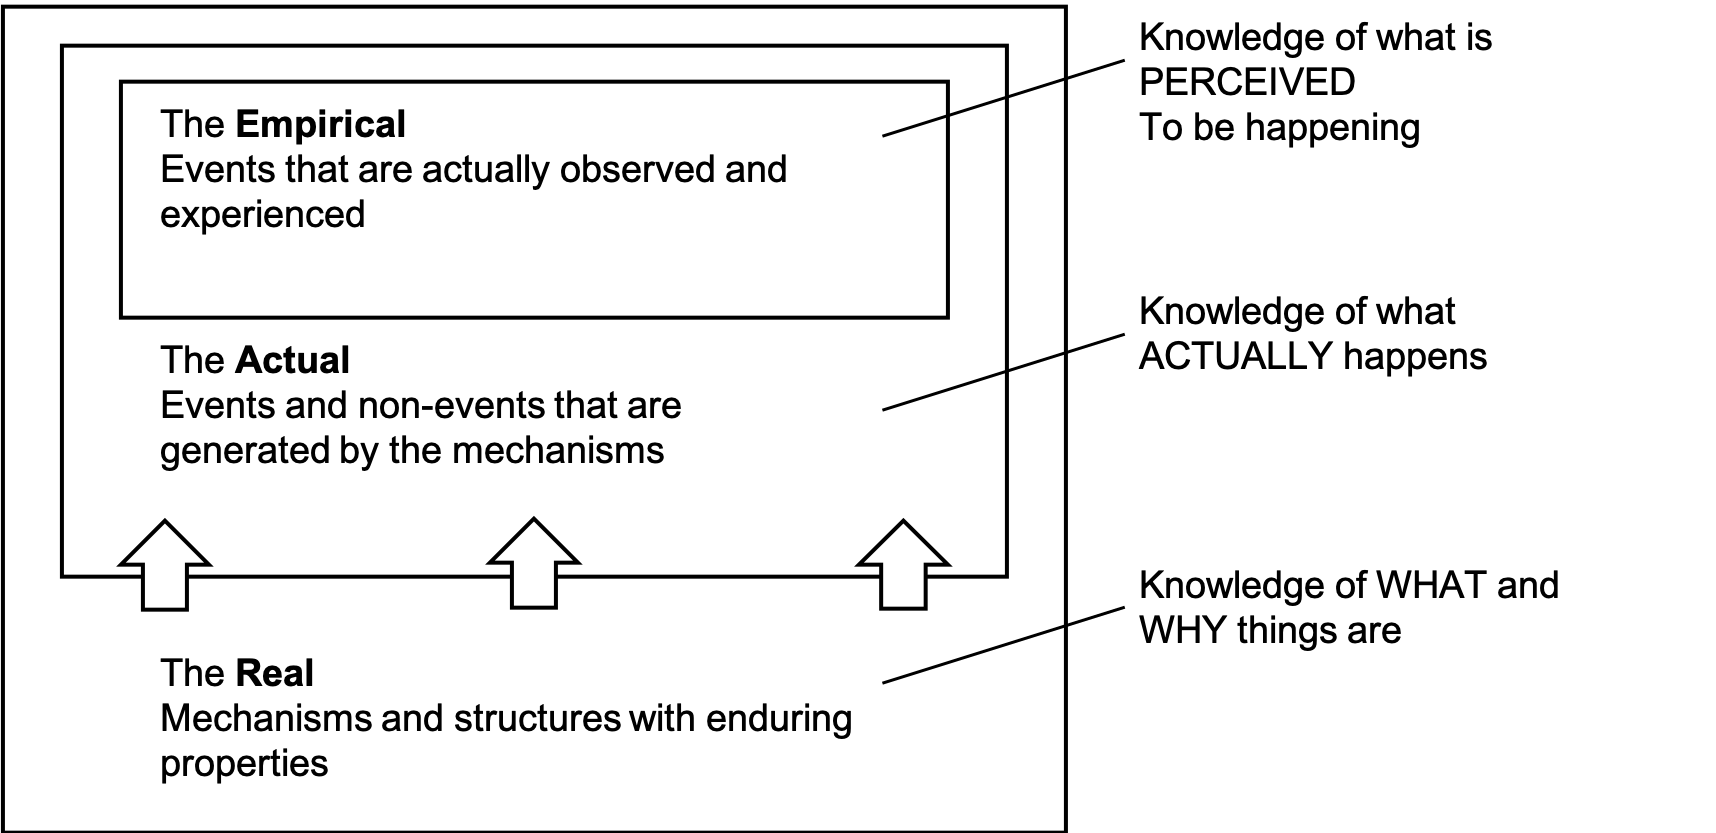
\includegraphics[width=0.9\linewidth]{Images/stratified_reality.png}
\caption[The stratified ontology of critical realism]{The stratified ontology of critical realism \citep{bhaskar2013realist,mingers2006realising}.}
\label{fig:stratified_reality}
\end{figure}

The critical realist applies the logic of retroduction to discover the interacting mechanisms and structures that may explain events \citep{sayer1999realism,wynn2012principles}. Retroduction suggests new ideas or explanations, some of which may, after testing by induction, turn out to be true (Figure \ref{fig:retroduction}). These mechanisms or structures can be physical, social, or psychological, and may not be directly observable except in terms of their effects (e.g. the configuration of network structures) \citep{mcavoy2018critical}. The primary goal of critical realism is to explain events through reference to these structures and mechanisms and the effects they can have across all three levels of reality \citep{wynn2012principles,fletcher2017applying}. \medskip

\begin{figure}[h!]
\centering
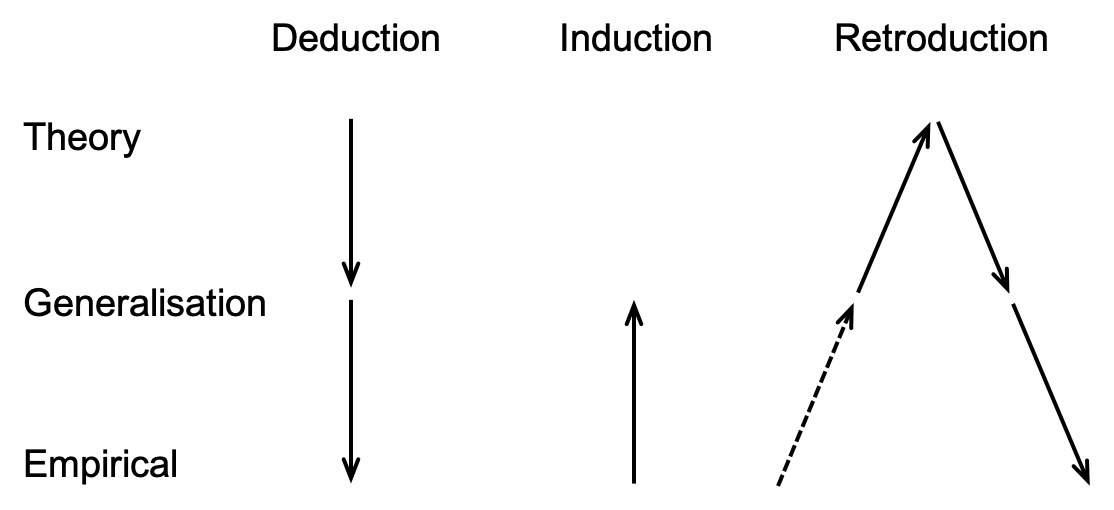
\includegraphics[width=0.7\linewidth]{Images/retroduction.png}
\caption[Logic of deduction, induction and retroduction]{Logic of deduction, induction and retroduction. Deduction is typically used to prove or disprove theory. Induction is used to generalise human experiences. Retroduction combines inductive and deductive reasoning to understand causal mechanisms as objectively as possible \citep{saether1998retroduction}.}
\label{fig:retroduction}
\end{figure}

\subsection{Justification for a critical realist approach}

This thesis aims to investigate mechanisms and structures that affect tacit knowledge sharing in open innovation. Though we can quantify social ties between participants and test hypotheses about tie formation in a positivist manner, this cannot account for external or experiential factors that influence tie formation. We need a combination of quantitative and qualitative methods to obtain a complete understanding of the mechanisms and structures affecting tacit knowledge sharing in open innovation. \medskip

Combining quantitative and qualitative methods is fraught because of the complex ontological and epistemological issues involved \citep{giddings2006mixed,mcevoy2006critical}. Methodological purists tend to be absolutist and argue strongly in favour of their preferred methodology. For them, quantitative and qualitative methods rely on mutually exclusive assumptions and are thus incommensurable \citep{greene2008mixed}. Methodological pragmatists, on the other hand, accept that assumptions can be mutually exclusive but assert that researchers should use whatever methods are needed to obtain useful results, even though this involves alternating between paradigms. The logic of methodological pragmatists is that neither quantitative nor qualitative methods alone are sufficient to develop a complete analysis \citep{mcevoy2006critical,creswell2013research}. Applying a pragmatic approach can be very challenging, especially when attempting to make sense of discordant data collected under different epistemological assumptions \citep{johnson2004mixed,giddings2006mixed}. Any study that involves mixing methods must reconcile ontological and epistemological differences to ensure findings are both credible and valid \citep{zachariadis2013methodological}. \medskip

The stratified ontology of critical realism allows for the \enquote{legitimate} combination of qualitative and quantitative methods. Table \ref{tab:mm_critical_realism} lists reasons for mixing methods in critical realism. In the case of this study, the quantitative analysis tested psychosocial theories to explain significant network effects. The quantitative analysis was \textit{complimented} by qualitative analysis of semi-structured interviews that allowed deeper exploration of the mechanisms and structures affecting tacit knowledge sharing in open innovation partnerships. Applying the logic of retroduction provided a more \textit{complete}, \textit{expansive} and \textit{diverse} picture of the mechanisms and structures affecting tacit knowledge sharing. \medskip

\begin{sidewaystable}[p]
\centering
\resizebox{0.9\textwidth}{!}{%	
\begin{threeparttable}
\footnotesize
\setlength{\tabcolsep}{6pt}
\renewcommand{\arraystretch}{1}
\caption[Reasons for mixing methods in critical realism]{Reasons for mixing methods in critical realism \citep{zachariadis2013methodological}.}
\label{tab:mm_critical_realism}
\begin{tabular}{p{4cm}p{8cm}p{8cm}}
\toprule
\multicolumn{1}{c}{\textbf{Goal}} & \multicolumn{1}{c}{\textbf{Description}} & \multicolumn{1}{c}{\textbf{Critical realist implication}} \\ \midrule
Complementarity & Mixed methods are used in order to gain complementary views about the same phenomena or events & Different levels of abstraction of a multi\hyp{}layered world demand different methods \\
Completeness & Mixed methods research design is used to ensure a complete picture (as detailed as possible) of the phenomenon under study & Requires meta-theoretical considerations \\
Developmental & Inferences of one type of research are being used as questions for another type of research & This being part of the retroductive approach of critical realism, inferences need to hypothesise about the causal mechanisms whose recovery will then inspire additional research \\
Expansion & Mixed methods are being implemented in order to provide explanations or expand the understanding obtained in previous research & Quantitative methods can be used to guide qualitative research which (subject to the context) is more capable of uncovering generative mechanisms \\
Confirmation & Mixed methods are used in order to confirm the findings from another study & Epistemic fallacy occurs when trying to validate qualitative results with quantitative methods \\
Compensation & The weakness of one method can be compensated by the use of another & The weaknesses of different methods are recognised so alternative methods can be used to compensate \\
Diversity & Mixed methods are used in order to obtain divergent views on the same phenomena & Different levels of abstraction of a multi- layered world demand different methods \\ \bottomrule
\end{tabular}\end{threeparttable}
%
}
\end{sidewaystable}

\subsection{Case-based research}

A case study involves detailed examination of a particular case or set of cases within a real-world context \citep{crowe2011case}. It is an established research design used extensively in a wide variety of disciplines. The case study approach lends itself well to capturing information on more explanatory \textquote{how}, \textquote{what} and \textquote{why} questions \citep{crowe2011case}. How one approaches a case study depends on one's epistemological standpoint. For example, \citet{eisenhardt1989building} argues that case studies are a good way to develop social theories. She advocates inductive theory-building research to highlight associations between constructs and variables that can be tested. Her approach seeks to establish regularities rather than the reasons behind them i.e. it emphasises generalisation over context \citep{welch2011theorising}. \citet{yin2009case}, on the other hand, prefers a more deductive approach to case studies. He thinks case studies are well-suited to test the validity of existing theories. His approach discounts contextual factors that may affect causal relationships \citep{welch2011theorising}. \citet{stake2005qualitative} argues that generalising the results of case studies is too simplistic and deterministic. He thinks the true value of case studies lies in understanding the uniqueness of each case. For him, it is all about understanding different contexts. \citet{welch2011theorising} argue that a critical realist approach offers a high degree of contextualisation without sacrificing the goal of causal explanation. Contextualised explanations can provide novel theoretical accounts that incorporate rather than deny complexity \citep{ragin2009reflections}. Table \ref{tab:welch_cases} highlights how the different case study approaches differ.  \medskip

\begin{sidewaystable}
\centering
\caption[Case study paradigms]{Case study paradigms. After \citet{welch2011theorising}.}
\label{tab:welch_cases}
\resizebox{\textwidth}{!}{%
\begin{tabular}{@{}p{5.5cm}p{5.5cm}p{5.5cm}p{5.5cm}p{5.5cm}@{}}
\toprule
Dimension &
  Inductive theory building &
  Natural experiment &
  Interpretive sense-making &
  Contextualised explanation \\ \midrule
Philosophical orientation &
  Positivist (empiricism) &
  Positivist (falsification) &
  Interpretive/ constructionist &
  Critical realist \\
Nature of research process &
  Objective search for generalities &
  Objective search for causes &
  Subjective search for meaning &
  Subjective search for causes \\
Case study outcome &
  Explanation in the form of testable propositions &
  Explanation in the form of cause-effect linkages &
  Understanding of actor's subjective experiences &
  Explanation in the form of causal mechanisms \\
Strength of case study &
  Induction &
  Internal validity &
  Rich description &
  Causes-of-effects explanations \\
Attitude to generalisation &
  Generalisation to population &
  Generalisation to theory (analytic generalisation) &
  Particularisation not generalisation &
  Contingent and limited generalisations \\
Nature of causality &
  Regularity model: proposing associations between events (weak form of causality) &
  Specifying cause effect relationships (strong form of causality) &
  Too simplistic and deterministic a concept &
  Specifying causal mechanisms and the contextual conditions under which they work (strong form of causality) \\
Treatment of context &
  Contextual description a first step only &
  Causal relationships are isolated from the context of the case &
  Contextual description necessary for understanding &
  Context integrated into explanation \\
Primary advocate &
  \citet{eisenhardt1989building} &
  \citet{yin2009case} &
  \citet{stake2005qualitative} &
  \citet{ragin2009reflections,bhaskar2013realist} \\ \bottomrule
\end{tabular}%
}
\end{sidewaystable}[]

\subsection{Mixed-methods research design}

This thesis uses a case-based mixed-method research design to unpack the social mechanisms and structures that shape tacit knowledge exchange ties in three open innovation partnerships. Figure \ref{fig:mm} outlines the different research stages of this study. The first step identified research gaps in the open innovation literature. These informed the research questions that are the focus of this study. The next step was to apply a critical realist research process to identify critical social mechanisms affecting tacit knowledge exchanges in open innovation partnerships, their impact, and how these are activated \citep{mcavoy2018critical}. \medskip

\begin{figure}[p]
\centering
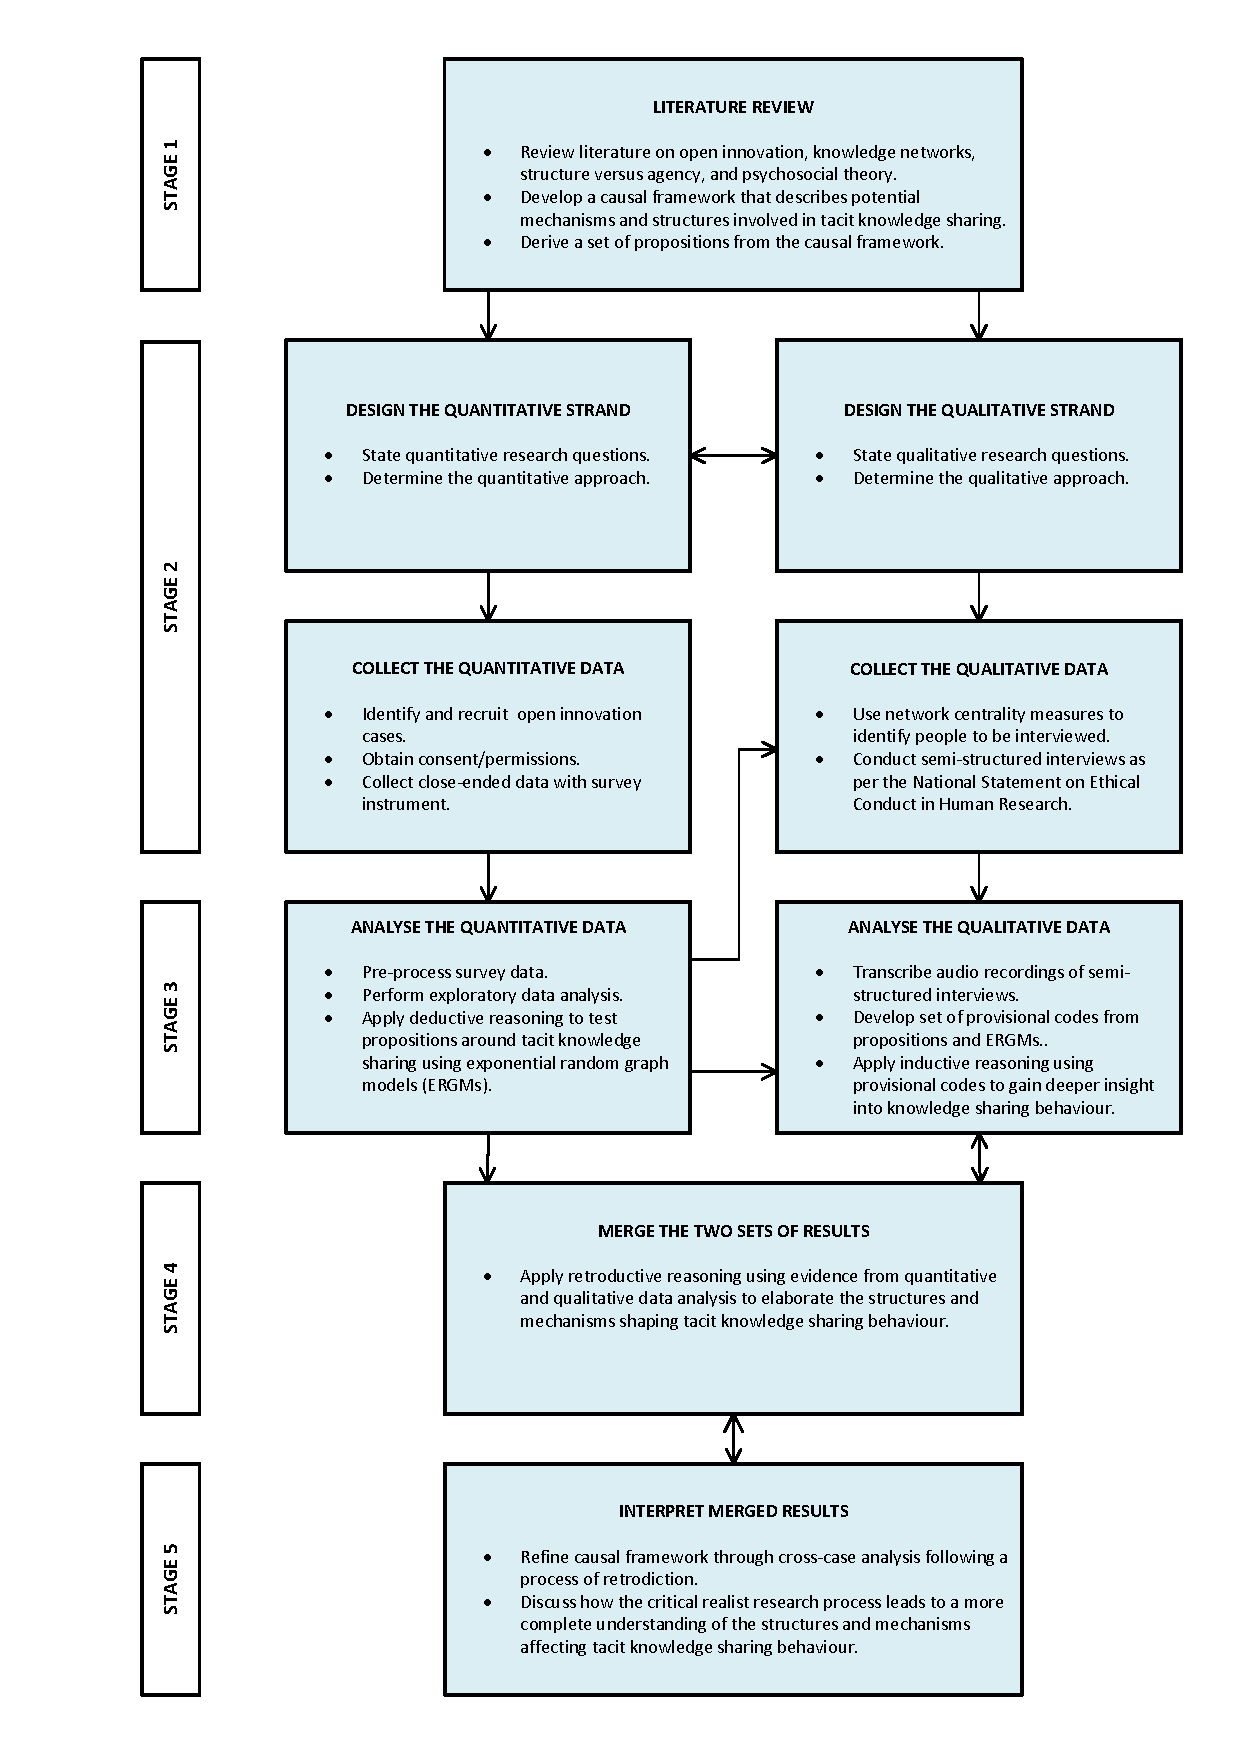
\includegraphics[width = 1.0\textwidth]{Images/mm.pdf}
\caption[Mixed method research design]{Mixed method critical realist research design.}
\label{fig:mm}
\end{figure}

Determining causal mechanisms in social network analysis is difficult because of the confounding nature of endogenous and exogenous network effects \citep{rogowski2012estimating,forastiere2018estimating}. Exponential random graph models (ERGMs) are a class of statistical model for social networks that allow simultaneous testing of multiple hypotheses about network structure and tie formation. Models represent an accumulation of local network configurations (also referred to as subgraphs, motifs, or microstructures) that build the global structure of the network \citep{robins2013tutorial}. Network configurations are assumed to represent underlying social processes or mechanisms \citep{lusher2013exponential}. A combination of social and psychological theories was used to predict purely structural network effects (reciprocity, popularity and activity spread, simple as well as multiple connectivity, transitive closure), actor-relation effects (sender/receiver, homophily), and actor-brokerage effects (different broker roles). While such quantitative analysis can disambiguate potentially confounding network effects, it cannot account for unobserved contextual or experiential factors that may affect network structures in open innovation partnerships. Hence, the next step in the critical realist research process is to apply retroduction to develop a more robust causal framework for each case. In the case of this study, the process of retroduction relied on evidence from the exponential random graph models and semi-structured interviews. It is important to note that with cross-sectional studies, such as this one, there is a limit to what one can infer about causal mechanisms. \medskip

The final step in the critical realist research process involves combining the causal frameworks for each case to create a cross\hyp{}case causal framework. Differences between cases are reconciled using retrodiction to create more robust explanations of mechanisms \citep{mcavoy2018critical}. \medskip

\section{Ethics clearance}

As this thesis deals with human participants, it was subject to the ethical guidelines contained in the Australian National Statement on Ethical Conduct in Human Research \citep{national2007national}. Formal ethics approval from both the Commonwealth Scientific and Industrial Research Organisation and Swinburne University of Technology was required before any data could be collected. Approval hinged on individual participants being sufficiently informed to give consent, allowing information about themselves to be used in this study. An application for ethics clearance was submitted to the ethics committees at both organisations. The application included a brief description of this study, a plain language information sheet for participants, a blank consent form, and a list of questions to be included in an online survey. Both committees deemed this study low-risk and allowed the collection and subsequent analysis of data to proceed, subject to standard terms and conditions as per the National Statement on Ethical Conduct in Human Research (the ethics approval may be found in Appendix A). These include alerting both committees to any changes in data collection procedures and reporting any complaints or issues raised by participants. None of the study participants raised any issues with the conduct of this study. 

\section{Research participants}

Finding appropriate candidates for open innovation case studies was challenging. This thesis is part of a broader initiative looking at innovation in the food and agriculture sector. Potential candidates were identified using leads provided by agricultural consultants, university researchers, government agencies, and non-governmental organisations. Most of the firms approached were not that keen on outsiders observing how they went about open innovation. Some firms argued their inter-organisational relationships were a trade-secret and did not want to risk anyone finding out about their strategic or commercial intentions. Other firms felt this study would consume too much their time or be too disruptive to their operations. Ultimately, the recruitment of cases relied on a combination of perseverance and goodwill. Altogether three cases were recruited for this study. 

\section{Quantitative procedures}

\subsection{Data collection}

Each case followed the same procedure for collecting and analysing quantitative data. For each case, the primary contact person (usually the project instigator) was asked to compile a list of people directly involved in the effort. An online survey was employed to collect quantitative data. The survey captured demographic information about respondents, whom they related to in the collaboration, and how they perceive themselves.\medskip

Any missing data impacts negatively on network studies. Hence this study aimed for a 100\% survey response rate. The primary contact person was asked to strongly encourage everybody on their list to participate in this study. 

\subsubsection{Questionnaire design}

The online survey was kept short as an inducement to complete the survey and to avoid responder fatigue \citep{crawford2001web,evans2005value,van2006conducting}. An informal poll among workplace colleagues at the Commonwealth Scientific Industrial Research Organisation (CSIRO) indicated that an online survey should take no longer than 15 or so minutes to complete. With this limitation in mind, the survey questionnaire was designed having three parts. The first part captured demographic information about the respondent, namely their age, gender, occupation, level and field of education, workplace postcode, relevant work experience, and current job tenure. Relevant work experience is essential as this is the primary source of useful tacit knowledge \citep{nonaka1995knowledge,sternberg1999tacit}. Response options for categorical questions were based on the Australian and New Zealand Standard Classification of Occupations \citep{pink2009anzsco} and the Australian Standard Classification of Education \citep{trewin2000australian}. Respondents were also asked to state their role in the open innovation partnership. \medskip

The second part of the questionnaire captured information about specific social relationships. Respondents were asked to name people in the open innovation collaboration they received knowledge and ideas from, felt they could trust, they reported to, and have worked with before (see Figure \ref{ng} for list of the name-generator and name-interpreter questions). \bigskip

\begin{figure}[p]
\centering
\label{ng}
\caption[Name-generator/interpreter questions]{Name-generator (NG) and name-interpreter (NI) questions.}
\begin{tcolorbox}
\begin{itemize}
    \item[\textbf{NG 1}] \textit{Name people who provide you with useful knowledge that helps you accomplish your tasks in this collaboration.}
    \begin{itemize}
        \item[\textbf{NI 1-1}] \textit{How much of the knowledge provided by this person is documented?}
        \item[\textbf{NI 1-2}] \textit{How complex is the knowledge provided by this person?}
        \item[\textbf{NI 1-3}] \textit{How much time does this person spend demonstrating their knowledge to me?}
    \end{itemize}
    \item[\textbf{NG 2}] \textit{Name people who help you come up with new ideas or novel solutions to hard problems in this collaboration.}
    \item[\textbf{NG 3}] \textit{Name people who help you transform ideas into product, process or service concepts for further development and commercialisation in this collaboration.}
    \item[\textbf{NG 4}] \textit{Name people in the collaboration you can share ideas, feelings and hopes with. These are people with whom you have made a considerable emotional investment in your working relationship. You can talk freely with them about the difficulties you are having at work. They will listen and respond in a constructive, caring way. You would share a sense of loss with them if you could no longer work together.}
    \item[\textbf{NG 5}] \textit{Name people in the collaboration you consider professional, competent, and dedicated. You can count on them not to make your job harder by careless work. They have the trust and respect of their colleagues, including those who are not friends.} 
    \item[\textbf{NG 6}] \textit{Name people you formally report to in this collaboration.}
    \item[\textbf{NG 7}] \textit{Name people in this collaboration you have worked and interacted with prior to this collaboration getting underway.}
\end{itemize}
\end{tcolorbox}
\end{figure}

Respondents could select names from a drop-down list or add names of people missing from the list. Asking respondents whom they receive knowledge and ideas from, rather than whom they share knowledge or generate ideas with, was a deliberate move to avoid them nominating everybody in the drop\hyp{}down list. By asking respondents to nominate whom they received knowledge and ideas from required them to think more carefully about their response. Respondents also had to indicate how much of the knowledge provided to them was tacit. Tacit knowledge may be characterised in terms of \enquote{complexity}, \enquote{codifiability}, and \enquote{observability} \citep{winter1987knowledge,zander1995knowledge,cavusgil2003tacit}. Any knowledge that is complex, poorly encoded, and mostly acquired through observation is considered to be predominantly tacit. For each knowledge provider, respondents had to rate how complex was the knowledge provided to them, to what extent was the knowledge documented, and how much direct observation was required to obtain the knowledge on a 10\hyp{}point scale. \medskip 

The third part of the questionnaire aimed to build a psychological profile of the respondent in terms of personality, self-efficacy, organisational identification, and work motivation. Respondents had to rate their level of agreement with several statements about themselves,  using a 10-point scale. Items from an ultra-shortened version of the \enquote{Big Five Inventory} was used to profile personality. The BFI-10 scale uses two items to measure each of the big five personality traits \citep{rammstedt2007measuring}. Only three personality traits positively correlated with knowledge sharing were profiled, namely \enquote{agreeableness}, \enquote{conscientiousness}, and \enquote{openness to experience} \citep{matzler2008personality,matzler2011personality}. While the BFI-10 is reported to be a less reliable scale (agreeableness: $\alpha$ = 0.42, conscientiousness: $\alpha$ = 0.67, emotional stability: $\alpha$ = 0.78, extraversion: $\alpha$ = 0.79, openness: $\alpha$ = 0.50), it is sufficient for research settings with tight time-constraints \citep{rammstedt2007measuring}.\medskip

This study assessed self-efficacy in terms of how competent a person felt about doing their job, their sense of autonomy, and confidence in their ability to come up with creative ideas or solutions. Job competence and autonomy was profiled using statements from the \enquote{Measuring Empowerment Scale} \citep{spreitzer1995psychological}. Reported reliability of this scale is considered good (job competence: $\alpha$ = 0.81, self-determination: $\alpha$ = 0.81). The ability to come up with creative ideas or solutions was profiled using statements from the \enquote{Creative Self\hyp{}Efficacy Scale} \citep{tierney2002creative}. Past studies indicate this scale is reliable with reported $\alpha$ values between 0.74 and 0.91 \citep{tierney2002creative,gong2009employee,tierney2011creative,mittal2015transformational}.\medskip

The \enquote{Organisational Identification Scale} \citep{mael1992alumni} was used to assess how strongly the respondent identified with his or her work\hyp{}group, employer, and with the open innovation partnership. This scale has proved to be reliable in a variety of study settings with reported $\alpha$ values between 0.73 and 0.89 \citep{mael1992alumni,bergami2000self,knippenberg2000foci,van2008interactive}. Only one of the six items from the scale was used in this survey: \enquote{When someone criticises my organisation, it feels like an insult}. This item has the highest factor loading of all six items \citep{mael1992identifying} and was adapted to address identification with one's work-group, with one's employer, and with the partnership. Using all six items for each of these cases would have been impractical, given the time constraint in which to complete the survey. \medskip

Work motivation was measured using the 19-item \enquote{Multidimensional Work Motivation Scale} \citep{gagne2015multidimensional}. This scale is based on self-determination theory and has sub-scales for amotivation, extrinsic material regulation, extrinsic social regulation, introjected regulation, identified regulation, and intrinsic motivation. Reliability of the English version is good, with reported $\alpha$ values between 0.79 and 0.90. Items in the Multidimensional Work Motivation Scale were modified to suit the study context. For example, the scale has a stem question: \enquote{Why do you or would you put efforts into your current job?}. One response option is: \enquote{Because I personally consider it important to put efforts into this job}. This response was modified to read as thus: \enquote{I put effort into this collaboration because I personally consider it important to do so}. 

\subsubsection{Piloting of the survey}

For quality assurance, the online survey was piloted twice to check if questions were clear and not ambiguous and to establish how long it would take to complete an online survey. Ten people were involved in each pilot (the first pilot involved CSIRO colleagues, the second involved members of the Social Network Research Laboratory at Swinburne University of Technology). Apart from one question about trust, everybody in the first pilot reported no issues with clarity or ambiguity. One person felt the question asking respondents to name people in the partnership they trust was too judgemental. The question was subsequently modified to be less judgemental. Everybody involved in the second pilot was comfortable with the survey, although one person felt the invitation email was too long. Most of the people in each pilot completed the survey within 20 minutes. The only exceptions were people who took their time making detailed notes as they went through the survey. Table \ref{tab:self-report} in Appendix B lists the 59 items used in the online survey, together with associated response options and references.

\subsubsection{Survey procedure}

The list of people involved in each open innovation partnership also included their email addresses. Everybody on the list received an email invite to complete the web-based survey questionnaire. The email provided information about the study and included a unique link to the survey website (\url{http://www.onasurveys.com}). People could either ignore the email invitation or agree to take part in the survey by clicking on the URL link provided. Clicking on the URL link directed them to the survey website where they were asked to give consent to allow their responses to be used in this study. They could not progress with the online survey until consent was given.

\subsection{Social network analysis}

\subsubsection{Key concepts}

A social network is a way to conceptualise a social system in terms of the structure of relationships among social actors. Typically, a social network is represented as a mathematical graph with vertices and edges. Vertices represent actors (also referred to as nodes) and edges the ties (social connections or relations) between them (Figure \ref{fig:examples}). \medskip

\begin{figure}
    \centering
    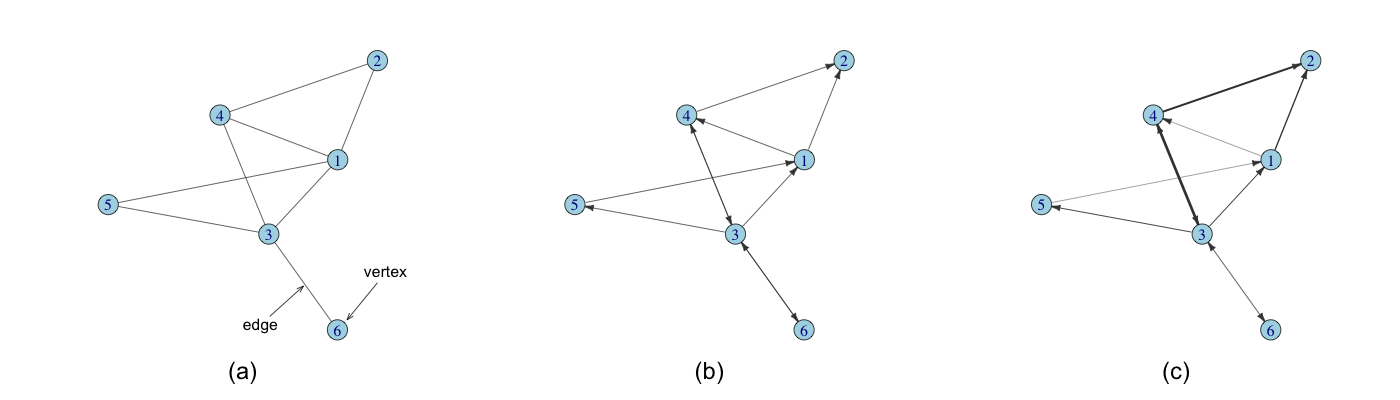
\includegraphics[width=1.0\linewidth]{Images/example_networks.png}
    \caption[Example networks]{Example network with (a) undirected binary ties, (b) directed binary ties, and (c) valued ties (edges are weighted according to some value).}
    \label{fig:examples}
\end{figure}

Actors may be distinguished using any combination of binary, categorical or continuous attributes. For example, consider an individual actor classified as female (binary attribute), who works for a particular organisation (categorical attribute), with a specific number of years of work experience (continuous attribute). Ties between actors can be measured as directed or undirected, and as binary or valued. Deciding whether to measure a tie as directed or undirected depends on the nature of the tie. For instance, ties indicating organisational affiliation are usually undirected, whereas authority is inherently directed \citep{borgatti2013analyzing}. \medskip
 
 A similarity tie is a type of continuous tie that shows a relation between two actors who share something in common (e.g. work at the same location, are affiliated to the same body, participate in the same event, or share a common attribute). Actors can have many different kinds of social relations, e.g. friendship, knowledge sharing, advice seeking, and reporting ties. Relational ties can also be affective (like or dislike another actor) or perceptual (belief about the other actor). Discrete ties refer to ties defined by specific social interactions (e.g. a transaction of some kind, attendance at the same event) and flows (e.g. communication or knowledge flows). \medskip

Ties are often interdependent insofar as the presence of one tie affects the presence of others. Without some form of dependence among ties, it is often difficult to explain the existence of specific social relations \citep{lusher2013exponential}. An example is a friendship tie, which usually develops in the presence of a pre-existing similarity tie (e.g. both actors share a common interest or work at the same place) or via an interaction tie (e.g. actors were introduced to each other at a specific event or worked together on a particular project). \medskip

\begin{figure}
    \centering
    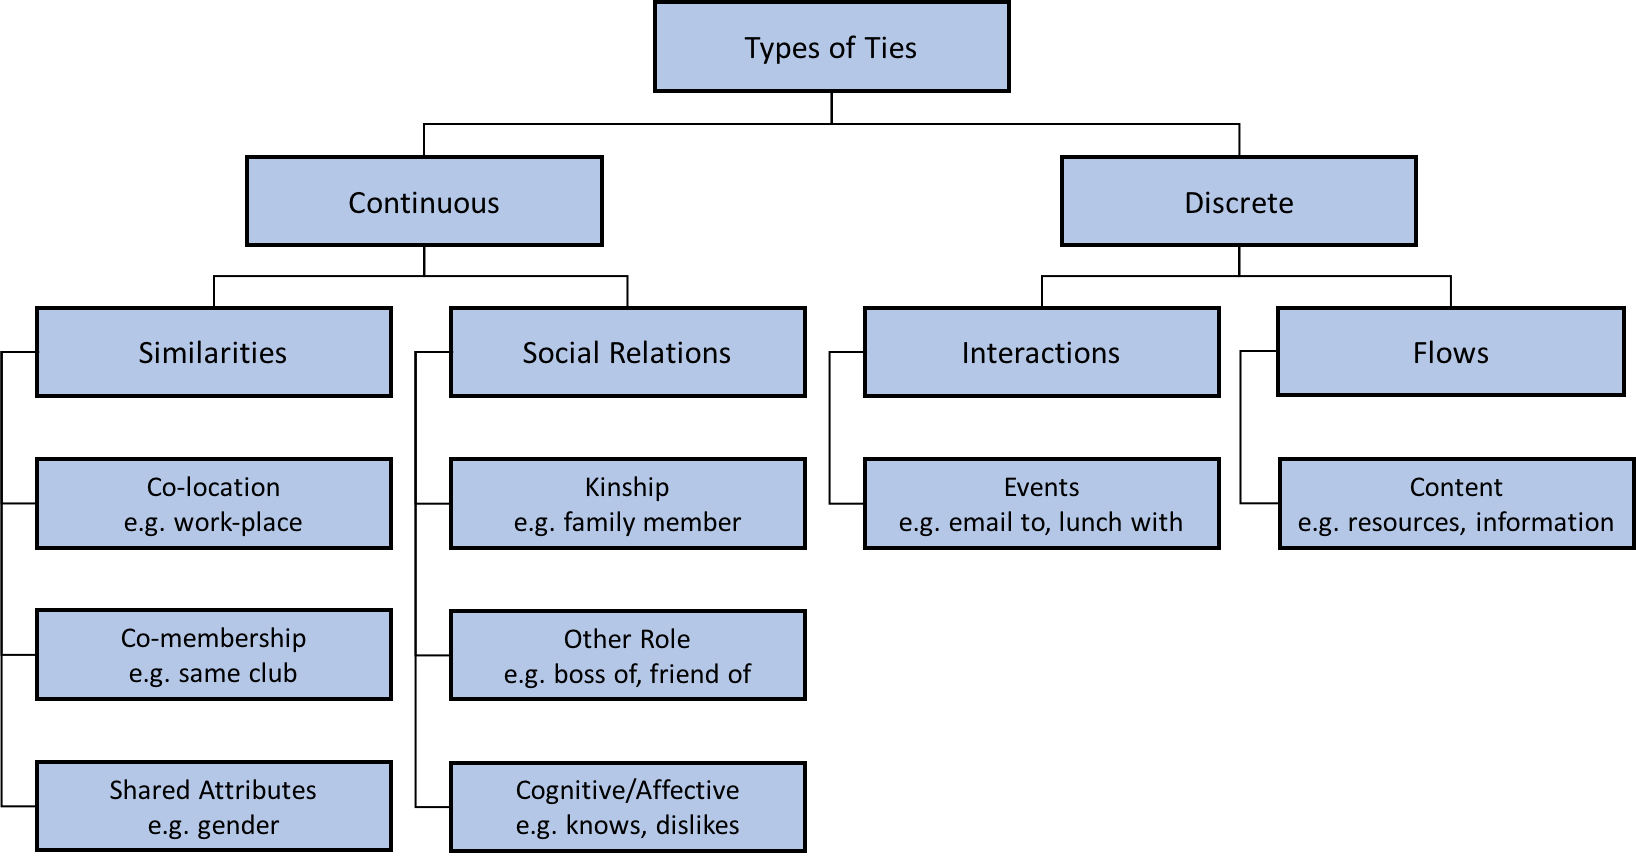
\includegraphics[width=0.9\linewidth]{tie_type}
    \caption[Different types of social ties]{Different types of social ties \citep{borgatti2013analyzing}.}
    \label{fig:tie_type}
\end{figure}

\subsubsection{Network data structures}

Edge lists and adjacency matrices are the most commonly used data structures for social networks. With an edge list, an edge between two actors $i$ and $j$ is denoted as $(i,j)$, so that a complete network with $n$ actors can be specified by giving the value $n$ and a list of edges. The edge list for the undirected binary network depicted in Figure \ref{fig:examples} would have $n = 6$ actors and edges (1,2), (1,3), (1,4), (1,5), (2,4), (3,4), (3,5), (3,6). A directed network has twice the number of total possible edges than an undirected network (directed network edges can be bi-directional). Thus, the edge list for the directed binary network depicted in Figure \ref{fig:examples} would have $n = 6$ actors and edges (1,2), (1,4), (3,1), (3,4), (3,5), (3,6), (4,2), (4,3), (5,1), (6,3). Although edge lists are an efficient way to represent networks, they are too cumbersome for computational operations \citep{newman2010networks}. \medskip

An adjacency matrix is a more efficient way to represent and manipulate social network data \citep{hummon1990computational}. For a social network, $X$, the adjacency matrix would be a $n \times n$ matrix with elements $X_{ij}$ representing how actor $i$ is tied to actor $j$. In the case of a binary network, the adjacency matrix is expressed as follows: 
\[
X_{ij} =
\begin{cases}
    1 & \text{if  } i \rightarrow j \\
    0 & \text{otherwise}
\end{cases}
\]
For an undirected network, $X_{ij}$ and $X_{ji}$ are equal. With a directed network, $X_{ij}$ and $X_{ji}$ are treated as different variables, either with the same or different values. For a directed binary network, values = 1 in the $i$th row of an adjacency matrix represent ties sent by actor $i$, and the values = 1 in the $j$th column of an adjacency matrix represent ties received by actor $j$. The adjacency matrix representing both the directed and undirected binary networks depicted in Figure \ref{fig:examples} would be expressed as: \bigskip
$$
X_{ij} =
\left \{
  \begin{tabular}{cccccc}
    0 & 1 & 0 & 1 & 0 & 0 \\
    0 & 0 & 0 & 0 & 0 & 0 \\
    1 & 0 & 0 & 1 & 1 & 1 \\
    0 & 1 & 1 & 0 & 0 & 0 \\
    1 & 0 & 0 & 0 & 0 & 0 \\
    0 & 0 & 1 & 0 & 0 & 0
  \end{tabular}
\right \}
$$ \medskip

In the case of non-binary or valued networks, the presence of a tie is indicated by some value (usually a real number, not equal to 0) that describes a property of the tie e.g. geographic proximity.

\subsubsection{Types of social network analysis}

Social network analysis aims to detect and interpret patterns of social ties between actors \citep{de2011exploratory}. Three core assumptions about patterned relations and their effects underpin social network analysis. First, structural relations are more important than actor attributes for understanding behaviour. For instance, an actor may be well-qualified to perform a specific task but is unable to do the task because the requisite relationships are not in place. Second, social networks shape and are shaped by the perceptions, beliefs, and actions of actors. Third, network structures are dynamic and continually evolving \citep{knoke2008social}. \medskip

Social network analysis can be either egocentric or socio-centric. Egocentric network analysis focuses on the structure of an actor's immediate network (the ego's network) and what this means for that actor \citep{chung2005exploring}. In contrast, socio-centric network analysis considers patterns of social interaction between all the actors in a predefined and bounded population \citep{provan2007interorganizational}. \medskip

This thesis used both descriptive and statistical network analysis techniques to analyse the socio-centric network structure of the three open innovation partnerships. The descriptive network analysis measured the centrality of actors and their brokerage roles in each open innovation partnership. This information was used to identify a subset of actors for follow-up semi-structured interviews (the subset included highly central as well as peripheral actors). The statistical network analysis used exponential random graph models (ERGMs) to examine the interdependence of knowledge sharing ties.

\subsubsection{Brief history of ERGMs}

Traditional methods for analysing social networks are primarily descriptive and not statistical in the sense of modelling random variation in how ties are formed among actors in a network \citep{harris2013introduction}. \citet{erdos1959random} formulated a simple random graph in which the proportion of observed ties out of all possible ties determines the probability of a tie forming between two actors. Simple random graphs are not very good at capturing observed network structures as they do not account for the social forces that influence tie formation \citep{harris2013introduction}. This led  \citet{holland1981exponential} to introduce a random graph model for directed graphs, where the probability of tie formation varies among actors according to their propensity to extend ties to other actors, and the propensity to have ties extended to them by other actors (referred to as a $p_1$ model). \medskip

While this was an improvement over simple random graphs, $p_1$ models do not reflect the interdependence among nodes (e.g. homophily and transitivity effects). Consequently,  \citet{frank1986markov} introduced a new generation of random graph model that assumes a form of dyadic dependence when ties do have actors in common (the Markov dependence assumption). Although it incorporated more of the structural characteristics found in observed networks, the model introduced by \citet{frank1986markov} does not include node attributes as covariates. \medskip

A major breakthrough came when \citet{wasserman1996logit} introduced a new model that assumes a more general conditional dependence between ties. Essentially, this model assumes the likelihood of any two ties existing at the same time is different from the combined likelihood of each tie being present. Their model allows for multiple dependence assumptions at both dyadic and node level(hence these models are referred to as $p^*$ models). \medskip

Statistically, an ERGM represents a probability distribution of graphs for a given set, where the probability of observing a graph is dependent on the presence of the various network configurations expressed by the model. Importantly, the unit of analysis in an ERGM is not the number of nodes, but the number of possible ties between all actors in the network ($n(n-1)$). Even with a small number of actors, an ERGM has sufficient statistical power to make inferences about how ties are formed \citep{lusher2013exponential}. \medskip

For a binary network, the probability of observing specific network configurations for a given set of actors \(n\) can be expressed as follows: $$ P(X = x) = \frac{\exp \left \{ \theta'z(x)  \right \}}{\kappa (\theta )} $$ where $P(x)$ indicates the probability of a given network, $\theta$ indicates a vector of model parameters, $z(x)$ is a vector of network statistics, and $\kappa$ is a normalising function to ensure a proper probability distribution across a set of random networks \citep{shumate2010exponential}. Network statistics $z(x)$ are counts of the estimated number of configurations in the network, or some function of those counts. The probability of the network depends on how many of those configurations are present and the parameters indicate the importance of each configuration \citep{lusher2013exponential}. Large positive parameters suggest that more configurations of that type are observed in the network than expected by chance alone \citep{robins2009closure}. \medskip

ERGMs are theory-driven in that their use requires the researcher to consider the complex, intersecting, and often competing theoretical reasons why particular social ties in the observed network exist \citep{lusher2020advances}. For instance, does a given network structure occur due to processes of homophily, reciprocity, transitivity, or through a combination of these? By including such parameters together in one model, a researcher can test certain hypotheses or propositions about tie formation relating to theory \citep{robins2007recent}. ERGMs can distinguish between ties formed due to actor attributes or whether an actor’s centrality is the result of being embedded within other purely structural network structures \citep{lusher2020advances}. Purely structural effects reflect self-organising or endogenous processes where ties form due to the presence or absence of other ties, e.g. reciprocity and transitive closure. Actor-relation effects refer to ties that form due to actor attributes. Homophily is an example of an actor-relation effect. Dyadic covariate effects refer to ties in one network being affected by ties in another network. A good example is the geographic separation between actors, which may affect the formation of relationships between them. Another example is advice seeking, which is more likely to occur in the presence of an existing friendship tie. \medskip

Alternative methods used to assess the effect of actor attributes on network structures, such as linear regression, are unable to make such distinctions and are thus more limited regarding the conclusions such methods can draw. One limitation of ERGMs is that the algorithms used to estimate model parameters often fail to converge (i.e. are unable to produce a stable set of parameter estimates). For this reason, ERGMs tend to be parsimonious, including only the most important configurations needed to answer specific research questions \citep{mcallister2017balancing,silk2017application}. 

\subsubsection{Data pre-processing}

The first step was to retrieve survey responses for each case from the \texttt{ONASurveys} website. Each case had its own Microsoft Excel\texttrademark\ workbook with two worksheets. The first worksheet contained demographic information about each respondent and their responses to the personality, self-efficacy, organisational identification, and work motivation scale items. The second worksheet listed for each respondent their nominated sources of knowledge and ideas, people they work with to realise ideas, trusted others, line or project managers, and individuals with whom they have previously worked. \medskip

Various \texttt{R} packages were used to pre-process data for social network analysis, generate network diagrams, and perform descriptive network analysis. These are listed in Appendix C (Table \ref{tab:r_scripts}). \texttt{R} is a popular cross-platform open-source software system for statistical computing \citep{core2018r}. Readers can access the \texttt{R} scripts used to pre-process, analyse and visualise data at \url{http://github.com/aterhorst/phd_scripts}. The exponential random graph modelling was done using \texttt{MPNet}, a Microsoft Windows\texttrademark\ application for statistical network analysis \citep{wang2014mpnet}. \medskip

Survey responses were loaded into \texttt{RStudio}, a free and open-source integrated development environment (IDE) for \texttt{R}, as two separate tabular data sets (i.e. a node table listing personal information about each respondent, and an edge table listing the different ways respondents relate to each other). The first step in the data tidying process involved fixing minor data-entry errors in the node table. Once data-entry errors were eliminated, the next step involved aggregating the personality, self-efficacy, organisational identification, and work motivation scale items. Aggregated scale items were re-scaled to be a fractional number between 0 and 1. \medskip

Respondents had to qualify the type of knowledge provided to them in terms of its complexity, observability, and level of encoding \citep{winter1987knowledge,zander1995knowledge,cavusgil2003tacit}. Knowledge sharing relations were valued on a scale of 0 to 1 by aggregating and re-scaling the three criteria to come up with a measure of knowledge tacitness. This allowed knowledge sharing relations to be split into two types, i.e. predominantly tacit and predominantly explicit knowledge sharing relations. Predominantly tacit knowledge (tacitness $> 0.5$) lacks documentation, is likely to be complex, and mostly acquired through observation. Predominantly explicit knowledge (tacitness $< 0.5$), on the other hand, tends to be well-documented, is not particularly complex, and requires little demonstration to be communicated. Although the edges of the predominantly tacit and a predominantly explicit knowledge network do not overlap, this thesis does not treat knowledge as a binary construct (as either completely tacit or totally explicit knowledge). This thesis assumes all knowledge has a tacit component. It uses a simple majority rule to differentiate knowledge according to its level of tacitness. \medskip

A multilayer network object was generated from the tidied node and edge data. Each layer in the network object represents a different set of relationships (tacit and explicit knowledge provider, idea contributor, cognition-based trust, affect-based trust, reporting, and historical relations). Given the survey asked respondents to name people in the partnership who (a) provided them with useful knowledge, and (b) contributed ideas to help them solve problems, the edges in both the knowledge provider and idea contributor layers were reversed to indicate the flow of knowledge and ideas. \medskip

The survey questionnaire asked respondents to enter their workplace postcodes. Geographic coordinates (longitude and latitude) were derived for each postcode using the \texttt{ggmap} package (the \texttt{geocode} function uses the Google Maps\texttrademark\ application programming interface (API) to do this). The spherical (also known as the \enquote{great circle}) distance between all survey respondents could then be calculated using the \texttt{geosphere} package (distances were expressed in kilometres). This information was added as an edge attribute in each network layer. \medskip

Adjacency matrices and corresponding node attributes were extracted from the multi-layer network object and saved as ASCII text files for exponential random graph modelling in \texttt{MPNet}. Apart from the valued adjacency matrix representing geographic separation between nodes (values = $log_e(\text{spherical distance(km)} + 1)$ between nodes), the adjacency matrices were binary in nature (0 = no edge between nodes, 1 = edge between nodes). 

\subsubsection{Exploratory data analysis}

The first thing to do with any survey data set is to get to know it. Not only does this allow one to become familiar with the data, it also helps reduce the workload during analysis \citep{cox2017translating}. Exploratory data analysis is about finding trends in the data, not so much about the strength of the evidence \citep{morgenthaler2009exploratory}. Usually, this involves applying various data visualisation techniques to explore the content and structure of the survey data. Insights gained from exploratory data analysis can help refine research questions, strengthen hypotheses, and improve model specifications \citep{jebb2017exploratory}. \medskip

Exploratory data analysis was used to assess responses to the survey scale items, check for significant correlations between survey items, profile the demographics of each case, and highlight central actors who provide and receive tacit and explicit knowledge as well as ideas in each case. Checking for a significant correlation between survey items involved combining the node tables for all three cases (to get a reasonable sample size). A correlation matrix was generated for the aggregated scale items using the \texttt{cor} function in the base \texttt{R} package. Significant correlations were visualised using the \texttt{corrplot} package in R \citep{wei2017corrplot}. Apart from highlighting interesting correlations between aggregated scale items, results from the correlation analysis helped guide the selection of actor attributes for the exponential random graph models. The graphical data analysis focused on the demographics of each case. This analysis included generating box-plots of age, job tenure, and work experience of actors (continuous variables) and rose-diagrams showing their level and field of education (categorical variables) using the \texttt{ggplot2} package in \texttt{R} \citep{wickham2016ggplot2}. Network diagrams depicting the predominantly tacit and predominantly explicit networks were generated using the \texttt{ggraph} package in \texttt{R} \citep{pedersen2019ggraph}. Nodes were sized according to their respective \enquote{Everett-Valente} brokerage scores \citep{everett2016bridging}. Edges were weighted according to the geographic distance between connected node pairs (expressed as $log_e(\text{spherical distance(km)} + 1)$). 

\subsubsection{Descriptive network analysis} \label{sss:descriptive_network_analysis}

The descriptive network analysis measured various centrality measures, namely in-degree, out-degree, and betweenness centrality for each actor in the tacit and explicit knowledge provider networks \citep{freeman1979centrality}. Also measured was the Everett-Valente brokerage score for each actor \citep{everett2016bridging}. The descriptive network analysis also measured the frequency of the five \citet{gould1989structures} broker roles in each network. \medskip 

In-degree centrality measures the number of ties directed towards an actor whereas out-degree centrality measures the number of ties directed away from an actor. Given the adjacency matrix of a directed network has the element $A_{ij} = 1$ for an edge from $j$ to $i$, in- and out-degrees can be expressed as: $$CD_i^{in} = \sum_{j = 1}^nA_{ij}, \,\,\,\,\,\, CD_j^{out} = \sum_{i = 1}^nA_{ij}$$ \noindent Put differently, in-degree centrality is the sum of column $j$ and out\hyp{}degree centrality is the sum of row $i$ in adjacency matrix $A_{ij}$ \citep{newman2010networks}. In-degree centrality is an indicator of an actor's ability to acquire knowledge, whereas out-degree centrality is an indicator of an actor's knowledge sharing activity. Betweenness centrality measures the extent to which an actor lies on paths between other actors: $$ CB_i=\sum_{i < k}\frac{g_{jik}}{g_{jk}} $$ where $b_i$ is the betweenness centrality for actor $i$, $g_{jik}$ is the number of shortest paths connecting $j$ and $k$ through $i$, and $g_{jk}$ is the total number of shortest paths connecting $j$ and $k$ \citep{freeman1979centrality}. Actors with high betweenness centrality are well\hyp{}positioned to control the flow of information or resources in a network \citep{everett2016bridging}. However, network size moderates the ability of actors to control information and resource flows (larger networks offer more alternative paths, limiting the control of actors). Hence, this study uses a modified betweenness centrality measure known as the \enquote{Everett-Valente} brokerage score that accounts for network size and isolated nodes \citep{everett2016bridging}. In the case of a directed network, as long as $CB_i \neq 0$, the incoming and outgoing Everett-Valente brokerage scores are calculated as follows: \medskip

$$\textit{in-EV-brokerage}_i = \frac{CB_i + j}{CD_i^{in}},  \,\,\,\,\,\, \textit{out-EV-brokerage}_i = \frac{CB_i + k}{CD_i^{out}} $$ \medskip

\noindent where $j$ is the number of vertices that can reach vertex $i$, and $k$ is the number vertices that $i$ can reach. Nodes depicted in the network diagrams were sized using the average of the incoming and outgoing brokerage measures: \medskip

$$ \textit{EV-Brokerage}_i = \frac{\textit{in-EV-Brokerage}_i + \textit{out-EV-Brokerage}_i}{2} $$ \medskip

To compute \citet{gould1989structures} broker roles, the tacit and explicit knowledge networks were extracted from the multi-layer network object and saved as a separate \texttt{network} objects \citep{butts2008network} using the \texttt{intergraph} package \citep{bojanowski2015intergraph}. The \texttt{brokerage} function in the R \texttt{sna} package \citep{butts2016sna} was then used to tally broker roles in each network. 

\subsubsection{Statistical network analysis}

Each case involved two sets of ERGMs. One set of ERGMs tested propositions about the role of motivation, trust, and power in tacit and explicit knowledge exchanges, while the other set examined the significance of different broker roles in each case. The propositions and exploratory analysis guided choosing which actor-relation effects to include in the first set of ERGMs. Apart from modelling each case separately, the cases were modelled together in one single ERGM. Modelling the cases in a single ERGM assumes the same endogenous and exogenous processes apply in all cases \citep{kalish2013brain}. Because the cases are unrelated to each other, the single ERGM used \enquote{structural zeros} to ensure that only between-case ties and not within-case ties were modelled \citep{lusher2012trust}. Structural zeros indicate there are no ties in these parts of the combined network - there cannot be because there are no connections between cases (see Figure \ref{tab:combined}. Modelling each case separately and then together in one combined network allows one to obtain a more nuanced view of processes operating in each case and how these deviate from the more general perspective. \medskip

\begin{figure}[h]
\begin{subtable}[h]{\textwidth}
\centering
\fontsize{16}{28} \selectfont
\resizebox{0.6\textwidth}{!}{
\begin{tabular}{
>{\columncolor[HTML]{EFEFEF}}l 
>{\columncolor[HTML]{EFEFEF}}l 
>{\columncolor[HTML]{EFEFEF}}l 
>{\columncolor[HTML]{EFEFEF}}l 
>{\columncolor[HTML]{EFEFEF}}l 
>{\columncolor[HTML]{EFEFEF}}l 
>{\columncolor[HTML]{EFEFEF}}l 
>{\columncolor[HTML]{EFEFEF}}l 
>{\columncolor[HTML]{EFEFEF}}l 
>{\columncolor[HTML]{EFEFEF}}l 
>{\columncolor[HTML]{EFEFEF}}l 
>{\columncolor[HTML]{EFEFEF}}l 
>{\columncolor[HTML]{EFEFEF}}l 
>{\columncolor[HTML]{EFEFEF}}l 
>{\columncolor[HTML]{EFEFEF}}l 
>{\columncolor[HTML]{EFEFEF}}l 
>{\columncolor[HTML]{EFEFEF}}l 
>{\columncolor[HTML]{EFEFEF}}l 
>{\columncolor[HTML]{EFEFEF}}l 
>{\columncolor[HTML]{EFEFEF}}l 
>{\columncolor[HTML]{EFEFEF}}l 
>{\columncolor[HTML]{EFEFEF}}l 
>{\columncolor[HTML]{EFEFEF}}l 
>{\columncolor[HTML]{EFEFEF}}l }
\cellcolor[HTML]{FD6864}0 & \cellcolor[HTML]{FD6864}0 & \cellcolor[HTML]{FD6864}0 & \cellcolor[HTML]{FD6864}1 & \cellcolor[HTML]{FD6864}1 & \cellcolor[HTML]{FD6864}0 & \cellcolor[HTML]{FD6864}1 & \cellcolor[HTML]{FD6864}0 & 0 & 0 & 0 & 0 & 0 & 0 & 0 & 0 & 0 & 0 & 0 & 0 & 0 & 0 & 0 & 0 \\
\cellcolor[HTML]{FD6864}0 & \cellcolor[HTML]{FD6864}0 & \cellcolor[HTML]{FD6864}1 & \cellcolor[HTML]{FD6864}0 & \cellcolor[HTML]{FD6864}0 & \cellcolor[HTML]{FD6864}0 & \cellcolor[HTML]{FD6864}1 & \cellcolor[HTML]{FD6864}0 & 0 & 0 & 0 & 0 & 0 & 0 & 0 & 0 & 0 & 0 & 0 & 0 & 0 & 0 & 0 & 0 \\
\cellcolor[HTML]{FD6864}0 & \cellcolor[HTML]{FD6864}0 & \cellcolor[HTML]{FD6864}0 & \cellcolor[HTML]{FD6864}0 & \cellcolor[HTML]{FD6864}0 & \cellcolor[HTML]{FD6864}0 & \cellcolor[HTML]{FD6864}0 & \cellcolor[HTML]{FD6864}1 & 0 & 0 & 0 & 0 & 0 & 0 & 0 & 0 & 0 & 0 & 0 & 0 & 0 & 0 & 0 & 0 \\
\cellcolor[HTML]{FD6864}0 & \cellcolor[HTML]{FD6864}0 & \cellcolor[HTML]{FD6864}1 & \cellcolor[HTML]{FD6864}0 & \cellcolor[HTML]{FD6864}1 & \cellcolor[HTML]{FD6864}1 & \cellcolor[HTML]{FD6864}0 & \cellcolor[HTML]{FD6864}1 & 0 & 0 & 0 & 0 & 0 & 0 & 0 & 0 & 0 & 0 & 0 & 0 & 0 & 0 & 0 & 0 \\
\cellcolor[HTML]{FD6864}1 & \cellcolor[HTML]{FD6864}0 & \cellcolor[HTML]{FD6864}1 & \cellcolor[HTML]{FD6864}0 & \cellcolor[HTML]{FD6864}0 & \cellcolor[HTML]{FD6864}1 & \cellcolor[HTML]{FD6864}1 & \cellcolor[HTML]{FD6864}1 & 0 & 0 & 0 & 0 & 0 & 0 & 0 & 0 & 0 & 0 & 0 & 0 & 0 & 0 & 0 & 0 \\
\cellcolor[HTML]{FD6864}1 & \cellcolor[HTML]{FD6864}0 & \cellcolor[HTML]{FD6864}1 & \cellcolor[HTML]{FD6864}0 & \cellcolor[HTML]{FD6864}1 & \cellcolor[HTML]{FD6864}0 & \cellcolor[HTML]{FD6864}0 & \cellcolor[HTML]{FD6864}0 & 0 & 0 & 0 & 0 & 0 & 0 & 0 & 0 & 0 & 0 & 0 & 0 & 0 & 0 & 0 & 0 \\
\cellcolor[HTML]{FD6864}0 & \cellcolor[HTML]{FD6864}0 & \cellcolor[HTML]{FD6864}1 & \cellcolor[HTML]{FD6864}0 & \cellcolor[HTML]{FD6864}0 & \cellcolor[HTML]{FD6864}0 & \cellcolor[HTML]{FD6864}0 & \cellcolor[HTML]{FD6864}0 & 0 & 0 & 0 & 0 & 0 & 0 & 0 & 0 & 0 & 0 & 0 & 0 & 0 & 0 & 0 & 0 \\
\cellcolor[HTML]{FD6864}0 & \cellcolor[HTML]{FD6864}0 & \cellcolor[HTML]{FD6864}1 & \cellcolor[HTML]{FD6864}0 & \cellcolor[HTML]{FD6864}0 & \cellcolor[HTML]{FD6864}1 & \cellcolor[HTML]{FD6864}0 & \cellcolor[HTML]{FD6864}0 & 0 & 0 & 0 & 0 & 0 & 0 & 0 & 0 & 0 & 0 & 0 & 0 & 0 & 0 & 0 & 0 \\
0 & 0 & 0 & 0 & 0 & 0 & 0 & 0 & \cellcolor[HTML]{32CB00}0 & \cellcolor[HTML]{32CB00}1 & \cellcolor[HTML]{32CB00}1 & \cellcolor[HTML]{32CB00}1 & 0 & 0 & 0 & 0 & 0 & 0 & 0 & 0 & 0 & 0 & 0 & 0 \\
0 & 0 & 0 & 0 & 0 & 0 & 0 & 0 & \cellcolor[HTML]{32CB00}0 & \cellcolor[HTML]{32CB00}0 & \cellcolor[HTML]{32CB00}0 & \cellcolor[HTML]{32CB00}1 & 0 & 0 & 0 & 0 & 0 & 0 & 0 & 0 & 0 & 0 & 0 & 0 \\
0 & 0 & 0 & 0 & 0 & 0 & 0 & 0 & \cellcolor[HTML]{32CB00}1 & \cellcolor[HTML]{32CB00}1 & \cellcolor[HTML]{32CB00}0 & \cellcolor[HTML]{32CB00}0 & 0 & 0 & 0 & 0 & 0 & 0 & 0 & 0 & 0 & 0 & 0 & 0 \\
0 & 0 & 0 & 0 & 0 & 0 & 0 & 0 & \cellcolor[HTML]{32CB00}0 & \cellcolor[HTML]{32CB00}0 & \cellcolor[HTML]{32CB00}0 & \cellcolor[HTML]{32CB00}0 & 0 & 0 & 0 & 0 & 0 & 0 & 0 & 0 & 0 & 0 & 0 & 0 \\
0 & 0 & 0 & 0 & 0 & 0 & 0 & 0 & 0 & 0 & 0 & 0 & \cellcolor[HTML]{3166FF}0 & \cellcolor[HTML]{3166FF}0 & \cellcolor[HTML]{3166FF}0 & \cellcolor[HTML]{3166FF}1 & \cellcolor[HTML]{3166FF}1 & \cellcolor[HTML]{3166FF}0 & \cellcolor[HTML]{3166FF}0 & \cellcolor[HTML]{3166FF}0 & \cellcolor[HTML]{3166FF}0 & \cellcolor[HTML]{3166FF}0 & \cellcolor[HTML]{3166FF}0 & \cellcolor[HTML]{3166FF}0 \\
0 & 0 & 0 & 0 & 0 & 0 & 0 & 0 & 0 & 0 & 0 & 0 & \cellcolor[HTML]{3166FF}1 & \cellcolor[HTML]{3166FF}0 & \cellcolor[HTML]{3166FF}0 & \cellcolor[HTML]{3166FF}1 & \cellcolor[HTML]{3166FF}0 & \cellcolor[HTML]{3166FF}0 & \cellcolor[HTML]{3166FF}0 & \cellcolor[HTML]{3166FF}0 & \cellcolor[HTML]{3166FF}0 & \cellcolor[HTML]{3166FF}0 & \cellcolor[HTML]{3166FF}0 & \cellcolor[HTML]{3166FF}0 \\
0 & 0 & 0 & 0 & 0 & 0 & 0 & 0 & 0 & 0 & 0 & 0 & \cellcolor[HTML]{3166FF}1 & \cellcolor[HTML]{3166FF}0 & \cellcolor[HTML]{3166FF}0 & \cellcolor[HTML]{3166FF}0 & \cellcolor[HTML]{3166FF}0 & \cellcolor[HTML]{3166FF}1 & \cellcolor[HTML]{3166FF}0 & \cellcolor[HTML]{3166FF}0 & \cellcolor[HTML]{3166FF}0 & \cellcolor[HTML]{3166FF}0 & \cellcolor[HTML]{3166FF}0 & \cellcolor[HTML]{3166FF}1 \\
0 & 0 & 0 & 0 & 0 & 0 & 0 & 0 & 0 & 0 & 0 & 0 & \cellcolor[HTML]{3166FF}0 & \cellcolor[HTML]{3166FF}0 & \cellcolor[HTML]{3166FF}0 & \cellcolor[HTML]{3166FF}0 & \cellcolor[HTML]{3166FF}1 & \cellcolor[HTML]{3166FF}1 & \cellcolor[HTML]{3166FF}0 & \cellcolor[HTML]{3166FF}0 & \cellcolor[HTML]{3166FF}0 & \cellcolor[HTML]{3166FF}0 & \cellcolor[HTML]{3166FF}0 & \cellcolor[HTML]{3166FF}0 \\
0 & 0 & 0 & 0 & 0 & 0 & 0 & 0 & 0 & 0 & 0 & 0 & \cellcolor[HTML]{3166FF}0 & \cellcolor[HTML]{3166FF}0 & \cellcolor[HTML]{3166FF}0 & \cellcolor[HTML]{3166FF}0 & \cellcolor[HTML]{3166FF}0 & \cellcolor[HTML]{3166FF}0 & \cellcolor[HTML]{3166FF}0 & \cellcolor[HTML]{3166FF}0 & \cellcolor[HTML]{3166FF}0 & \cellcolor[HTML]{3166FF}0 & \cellcolor[HTML]{3166FF}0 & \cellcolor[HTML]{3166FF}0 \\
0 & 0 & 0 & 0 & 0 & 0 & 0 & 0 & 0 & 0 & 0 & 0 & \cellcolor[HTML]{3166FF}0 & \cellcolor[HTML]{3166FF}0 & \cellcolor[HTML]{3166FF}0 & \cellcolor[HTML]{3166FF}0 & \cellcolor[HTML]{3166FF}0 & \cellcolor[HTML]{3166FF}0 & \cellcolor[HTML]{3166FF}1 & \cellcolor[HTML]{3166FF}0 & \cellcolor[HTML]{3166FF}0 & \cellcolor[HTML]{3166FF}0 & \cellcolor[HTML]{3166FF}0 & \cellcolor[HTML]{3166FF}0 \\
0 & 0 & 0 & 0 & 0 & 0 & 0 & 0 & 0 & 0 & 0 & 0 & \cellcolor[HTML]{3166FF}0 & \cellcolor[HTML]{3166FF}0 & \cellcolor[HTML]{3166FF}0 & \cellcolor[HTML]{3166FF}0 & \cellcolor[HTML]{3166FF}0 & \cellcolor[HTML]{3166FF}0 & \cellcolor[HTML]{3166FF}0 & \cellcolor[HTML]{3166FF}0 & \cellcolor[HTML]{3166FF}0 & \cellcolor[HTML]{3166FF}0 & \cellcolor[HTML]{3166FF}0 & \cellcolor[HTML]{3166FF}1 \\
0 & 0 & 0 & 0 & 0 & 0 & 0 & 0 & 0 & 0 & 0 & 0 & \cellcolor[HTML]{3166FF}0 & \cellcolor[HTML]{3166FF}0 & \cellcolor[HTML]{3166FF}1 & \cellcolor[HTML]{3166FF}0 & \cellcolor[HTML]{3166FF}1 & \cellcolor[HTML]{3166FF}1 & \cellcolor[HTML]{3166FF}0 & \cellcolor[HTML]{3166FF}0 & \cellcolor[HTML]{3166FF}1 & \cellcolor[HTML]{3166FF}0 & \cellcolor[HTML]{3166FF}0 & \cellcolor[HTML]{3166FF}0 \\
0 & 0 & 0 & 0 & 0 & 0 & 0 & 0 & 0 & 0 & 0 & 0 & \cellcolor[HTML]{3166FF}0 & \cellcolor[HTML]{3166FF}0 & \cellcolor[HTML]{3166FF}0 & \cellcolor[HTML]{3166FF}0 & \cellcolor[HTML]{3166FF}0 & \cellcolor[HTML]{3166FF}0 & \cellcolor[HTML]{3166FF}0 & \cellcolor[HTML]{3166FF}0 & \cellcolor[HTML]{3166FF}0 & \cellcolor[HTML]{3166FF}1 & \cellcolor[HTML]{3166FF}0 & \cellcolor[HTML]{3166FF}1 \\
0 & 0 & 0 & 0 & 0 & 0 & 0 & 0 & 0 & 0 & 0 & 0 & \cellcolor[HTML]{3166FF}1 & \cellcolor[HTML]{3166FF}0 & \cellcolor[HTML]{3166FF}1 & \cellcolor[HTML]{3166FF}0 & \cellcolor[HTML]{3166FF}0 & \cellcolor[HTML]{3166FF}0 & \cellcolor[HTML]{3166FF}0 & \cellcolor[HTML]{3166FF}1 & \cellcolor[HTML]{3166FF}0 & \cellcolor[HTML]{3166FF}0 & \cellcolor[HTML]{3166FF}0 & \cellcolor[HTML]{3166FF}0 \\
0 & 0 & 0 & 0 & 0 & 0 & 0 & 0 & 0 & 0 & 0 & 0 & \cellcolor[HTML]{3166FF}0 & \cellcolor[HTML]{3166FF}0 & \cellcolor[HTML]{3166FF}0 & \cellcolor[HTML]{3166FF}0 & \cellcolor[HTML]{3166FF}1 & \cellcolor[HTML]{3166FF}0 & \cellcolor[HTML]{3166FF}1 & \cellcolor[HTML]{3166FF}0 & \cellcolor[HTML]{3166FF}0 & \cellcolor[HTML]{3166FF}0 & \cellcolor[HTML]{3166FF}0 & \cellcolor[HTML]{3166FF}0 \\
0 & 0 & 0 & 0 & 0 & 0 & 0 & 0 & 0 & 0 & 0 & 0 & \cellcolor[HTML]{3166FF}0 & \cellcolor[HTML]{3166FF}0 & \cellcolor[HTML]{3166FF}0 & \cellcolor[HTML]{3166FF}0 & \cellcolor[HTML]{3166FF}1 & \cellcolor[HTML]{3166FF}0 & \cellcolor[HTML]{3166FF}0 & \cellcolor[HTML]{3166FF}0 & \cellcolor[HTML]{3166FF}1 & \cellcolor[HTML]{3166FF}0 & \cellcolor[HTML]{3166FF}0 & \cellcolor[HTML]{3166FF}0
\end{tabular}
}
\caption{Combined network adjacency matrix.}
\label{tab:combined}
\end{subtable}
\newline
\vspace*{0.5 cm}
\newline
\begin{subtable}[h]{\textwidth}
\centering
\fontsize{16}{28} \selectfont
\resizebox{0.6\textwidth}{!}{
\begin{tabular}{
>{\columncolor[HTML]{EFEFEF}}l 
>{\columncolor[HTML]{EFEFEF}}l 
>{\columncolor[HTML]{EFEFEF}}l 
>{\columncolor[HTML]{EFEFEF}}l 
>{\columncolor[HTML]{EFEFEF}}l 
>{\columncolor[HTML]{EFEFEF}}l 
>{\columncolor[HTML]{EFEFEF}}l 
>{\columncolor[HTML]{EFEFEF}}l 
>{\columncolor[HTML]{EFEFEF}}l 
>{\columncolor[HTML]{EFEFEF}}l 
>{\columncolor[HTML]{EFEFEF}}l 
>{\columncolor[HTML]{EFEFEF}}l 
>{\columncolor[HTML]{EFEFEF}}l 
>{\columncolor[HTML]{EFEFEF}}l 
>{\columncolor[HTML]{EFEFEF}}l 
>{\columncolor[HTML]{EFEFEF}}l 
>{\columncolor[HTML]{EFEFEF}}l 
>{\columncolor[HTML]{EFEFEF}}l 
>{\columncolor[HTML]{EFEFEF}}l 
>{\columncolor[HTML]{EFEFEF}}l 
>{\columncolor[HTML]{EFEFEF}}l 
>{\columncolor[HTML]{EFEFEF}}l 
>{\columncolor[HTML]{EFEFEF}}l 
>{\columncolor[HTML]{EFEFEF}}l }
\cellcolor[HTML]{FD6864}1 & \cellcolor[HTML]{FD6864}1 & \cellcolor[HTML]{FD6864}1 & \cellcolor[HTML]{FD6864}1 & \cellcolor[HTML]{FD6864}1 & \cellcolor[HTML]{FD6864}1 & \cellcolor[HTML]{FD6864}1 & \cellcolor[HTML]{FD6864}1 & 0 & 0 & 0 & 0 & 0 & 0 & 0 & 0 & 0 & 0 & 0 & 0 & 0 & 0 & 0 & 0 \\
\cellcolor[HTML]{FD6864}1 & \cellcolor[HTML]{FD6864}1 & \cellcolor[HTML]{FD6864}1 & \cellcolor[HTML]{FD6864}1 & \cellcolor[HTML]{FD6864}1 & \cellcolor[HTML]{FD6864}1 & \cellcolor[HTML]{FD6864}1 & \cellcolor[HTML]{FD6864}1 & 0 & 0 & 0 & 0 & 0 & 0 & 0 & 0 & 0 & 0 & 0 & 0 & 0 & 0 & 0 & 0 \\
\cellcolor[HTML]{FD6864}1 & \cellcolor[HTML]{FD6864}1 & \cellcolor[HTML]{FD6864}1 & \cellcolor[HTML]{FD6864}1 & \cellcolor[HTML]{FD6864}1 & \cellcolor[HTML]{FD6864}1 & \cellcolor[HTML]{FD6864}1 & \cellcolor[HTML]{FD6864}1 & 0 & 0 & 0 & 0 & 0 & 0 & 0 & 0 & 0 & 0 & 0 & 0 & 0 & 0 & 0 & 0 \\
\cellcolor[HTML]{FD6864}1 & \cellcolor[HTML]{FD6864}1 & \cellcolor[HTML]{FD6864}1 & \cellcolor[HTML]{FD6864}1 & \cellcolor[HTML]{FD6864}1 & \cellcolor[HTML]{FD6864}1 & \cellcolor[HTML]{FD6864}1 & \cellcolor[HTML]{FD6864}1 & 0 & 0 & 0 & 0 & 0 & 0 & 0 & 0 & 0 & 0 & 0 & 0 & 0 & 0 & 0 & 0 \\
\cellcolor[HTML]{FD6864}1 & \cellcolor[HTML]{FD6864}1 & \cellcolor[HTML]{FD6864}1 & \cellcolor[HTML]{FD6864}1 & \cellcolor[HTML]{FD6864}1 & \cellcolor[HTML]{FD6864}1 & \cellcolor[HTML]{FD6864}1 & \cellcolor[HTML]{FD6864}1 & 0 & 0 & 0 & 0 & 0 & 0 & 0 & 0 & 0 & 0 & 0 & 0 & 0 & 0 & 0 & 0 \\
\cellcolor[HTML]{FD6864}1 & \cellcolor[HTML]{FD6864}1 & \cellcolor[HTML]{FD6864}1 & \cellcolor[HTML]{FD6864}1 & \cellcolor[HTML]{FD6864}1 & \cellcolor[HTML]{FD6864}1 & \cellcolor[HTML]{FD6864}1 & \cellcolor[HTML]{FD6864}1 & 0 & 0 & 0 & 0 & 0 & 0 & 0 & 0 & 0 & 0 & 0 & 0 & 0 & 0 & 0 & 0 \\
\cellcolor[HTML]{FD6864}1 & \cellcolor[HTML]{FD6864}1 & \cellcolor[HTML]{FD6864}1 & \cellcolor[HTML]{FD6864}1 & \cellcolor[HTML]{FD6864}1 & \cellcolor[HTML]{FD6864}1 & \cellcolor[HTML]{FD6864}1 & \cellcolor[HTML]{FD6864}1 & 0 & 0 & 0 & 0 & 0 & 0 & 0 & 0 & 0 & 0 & 0 & 0 & 0 & 0 & 0 & 0 \\
\cellcolor[HTML]{FD6864}1 & \cellcolor[HTML]{FD6864}1 & \cellcolor[HTML]{FD6864}1 & \cellcolor[HTML]{FD6864}1 & \cellcolor[HTML]{FD6864}1 & \cellcolor[HTML]{FD6864}1 & \cellcolor[HTML]{FD6864}1 & \cellcolor[HTML]{FD6864}1 & 0 & 0 & 0 & 0 & 0 & 0 & 0 & 0 & 0 & 0 & 0 & 0 & 0 & 0 & 0 & 0 \\
0 & 0 & 0 & 0 & 0 & 0 & 0 & 0 & \cellcolor[HTML]{32CB00}1 & \cellcolor[HTML]{32CB00}1 & \cellcolor[HTML]{32CB00}1 & \cellcolor[HTML]{32CB00}1 & 0 & 0 & 0 & 0 & 0 & 0 & 0 & 0 & 0 & 0 & 0 & 0 \\
0 & 0 & 0 & 0 & 0 & 0 & 0 & 0 & \cellcolor[HTML]{32CB00}1 & \cellcolor[HTML]{32CB00}1 & \cellcolor[HTML]{32CB00}1 & \cellcolor[HTML]{32CB00}1 & 0 & 0 & 0 & 0 & 0 & 0 & 0 & 0 & 0 & 0 & 0 & 0 \\
0 & 0 & 0 & 0 & 0 & 0 & 0 & 0 & \cellcolor[HTML]{32CB00}1 & \cellcolor[HTML]{32CB00}1 & \cellcolor[HTML]{32CB00}1 & \cellcolor[HTML]{32CB00}1 & 0 & 0 & 0 & 0 & 0 & 0 & 0 & 0 & 0 & 0 & 0 & 0 \\
0 & 0 & 0 & 0 & 0 & 0 & 0 & 0 & \cellcolor[HTML]{32CB00}1 & \cellcolor[HTML]{32CB00}1 & \cellcolor[HTML]{32CB00}1 & \cellcolor[HTML]{32CB00}1 & 0 & 0 & 0 & 0 & 0 & 0 & 0 & 0 & 0 & 0 & 0 & 0 \\
0 & 0 & 0 & 0 & 0 & 0 & 0 & 0 & 0 & 0 & 0 & 0 & \cellcolor[HTML]{3166FF}1 & \cellcolor[HTML]{3166FF}1 & \cellcolor[HTML]{3166FF}1 & \cellcolor[HTML]{3166FF}1 & \cellcolor[HTML]{3166FF}1 & \cellcolor[HTML]{3166FF}1 & \cellcolor[HTML]{3166FF}1 & \cellcolor[HTML]{3166FF}1 & \cellcolor[HTML]{3166FF}1 & \cellcolor[HTML]{3166FF}1 & \cellcolor[HTML]{3166FF}1 & \cellcolor[HTML]{3166FF}1 \\
0 & 0 & 0 & 0 & 0 & 0 & 0 & 0 & 0 & 0 & 0 & 0 & \cellcolor[HTML]{3166FF}1 & \cellcolor[HTML]{3166FF}1 & \cellcolor[HTML]{3166FF}1 & \cellcolor[HTML]{3166FF}1 & \cellcolor[HTML]{3166FF}1 & \cellcolor[HTML]{3166FF}1 & \cellcolor[HTML]{3166FF}1 & \cellcolor[HTML]{3166FF}1 & \cellcolor[HTML]{3166FF}1 & \cellcolor[HTML]{3166FF}1 & \cellcolor[HTML]{3166FF}1 & \cellcolor[HTML]{3166FF}1 \\
0 & 0 & 0 & 0 & 0 & 0 & 0 & 0 & 0 & 0 & 0 & 0 & \cellcolor[HTML]{3166FF}1 & \cellcolor[HTML]{3166FF}1 & \cellcolor[HTML]{3166FF}1 & \cellcolor[HTML]{3166FF}1 & \cellcolor[HTML]{3166FF}1 & \cellcolor[HTML]{3166FF}1 & \cellcolor[HTML]{3166FF}1 & \cellcolor[HTML]{3166FF}1 & \cellcolor[HTML]{3166FF}1 & \cellcolor[HTML]{3166FF}1 & \cellcolor[HTML]{3166FF}1 & \cellcolor[HTML]{3166FF}1 \\
0 & 0 & 0 & 0 & 0 & 0 & 0 & 0 & 0 & 0 & 0 & 0 & \cellcolor[HTML]{3166FF}1 & \cellcolor[HTML]{3166FF}1 & \cellcolor[HTML]{3166FF}1 & \cellcolor[HTML]{3166FF}1 & \cellcolor[HTML]{3166FF}1 & \cellcolor[HTML]{3166FF}1 & \cellcolor[HTML]{3166FF}1 & \cellcolor[HTML]{3166FF}1 & \cellcolor[HTML]{3166FF}1 & \cellcolor[HTML]{3166FF}1 & \cellcolor[HTML]{3166FF}1 & \cellcolor[HTML]{3166FF}1 \\
0 & 0 & 0 & 0 & 0 & 0 & 0 & 0 & 0 & 0 & 0 & 0 & \cellcolor[HTML]{3166FF}1 & \cellcolor[HTML]{3166FF}1 & \cellcolor[HTML]{3166FF}1 & \cellcolor[HTML]{3166FF}1 & \cellcolor[HTML]{3166FF}1 & \cellcolor[HTML]{3166FF}1 & \cellcolor[HTML]{3166FF}1 & \cellcolor[HTML]{3166FF}1 & \cellcolor[HTML]{3166FF}1 & \cellcolor[HTML]{3166FF}1 & \cellcolor[HTML]{3166FF}1 & \cellcolor[HTML]{3166FF}1 \\
0 & 0 & 0 & 0 & 0 & 0 & 0 & 0 & 0 & 0 & 0 & 0 & \cellcolor[HTML]{3166FF}1 & \cellcolor[HTML]{3166FF}1 & \cellcolor[HTML]{3166FF}1 & \cellcolor[HTML]{3166FF}1 & \cellcolor[HTML]{3166FF}1 & \cellcolor[HTML]{3166FF}1 & \cellcolor[HTML]{3166FF}1 & \cellcolor[HTML]{3166FF}1 & \cellcolor[HTML]{3166FF}1 & \cellcolor[HTML]{3166FF}1 & \cellcolor[HTML]{3166FF}1 & \cellcolor[HTML]{3166FF}1 \\
0 & 0 & 0 & 0 & 0 & 0 & 0 & 0 & 0 & 0 & 0 & 0 & \cellcolor[HTML]{3166FF}1 & \cellcolor[HTML]{3166FF}1 & \cellcolor[HTML]{3166FF}1 & \cellcolor[HTML]{3166FF}1 & \cellcolor[HTML]{3166FF}1 & \cellcolor[HTML]{3166FF}1 & \cellcolor[HTML]{3166FF}1 & \cellcolor[HTML]{3166FF}1 & \cellcolor[HTML]{3166FF}1 & \cellcolor[HTML]{3166FF}1 & \cellcolor[HTML]{3166FF}1 & \cellcolor[HTML]{3166FF}1 \\
0 & 0 & 0 & 0 & 0 & 0 & 0 & 0 & 0 & 0 & 0 & 0 & \cellcolor[HTML]{3166FF}1 & \cellcolor[HTML]{3166FF}1 & \cellcolor[HTML]{3166FF}1 & \cellcolor[HTML]{3166FF}1 & \cellcolor[HTML]{3166FF}1 & \cellcolor[HTML]{3166FF}1 & \cellcolor[HTML]{3166FF}1 & \cellcolor[HTML]{3166FF}1 & \cellcolor[HTML]{3166FF}1 & \cellcolor[HTML]{3166FF}1 & \cellcolor[HTML]{3166FF}1 & \cellcolor[HTML]{3166FF}1 \\
0 & 0 & 0 & 0 & 0 & 0 & 0 & 0 & 0 & 0 & 0 & 0 & \cellcolor[HTML]{3166FF}1 & \cellcolor[HTML]{3166FF}1 & \cellcolor[HTML]{3166FF}1 & \cellcolor[HTML]{3166FF}1 & \cellcolor[HTML]{3166FF}1 & \cellcolor[HTML]{3166FF}1 & \cellcolor[HTML]{3166FF}1 & \cellcolor[HTML]{3166FF}1 & \cellcolor[HTML]{3166FF}1 & \cellcolor[HTML]{3166FF}1 & \cellcolor[HTML]{3166FF}1 & \cellcolor[HTML]{3166FF}1 \\
0 & 0 & 0 & 0 & 0 & 0 & 0 & 0 & 0 & 0 & 0 & 0 & \cellcolor[HTML]{3166FF}1 & \cellcolor[HTML]{3166FF}1 & \cellcolor[HTML]{3166FF}1 & \cellcolor[HTML]{3166FF}1 & \cellcolor[HTML]{3166FF}1 & \cellcolor[HTML]{3166FF}1 & \cellcolor[HTML]{3166FF}1 & \cellcolor[HTML]{3166FF}1 & \cellcolor[HTML]{3166FF}1 & \cellcolor[HTML]{3166FF}1 & \cellcolor[HTML]{3166FF}1 & \cellcolor[HTML]{3166FF}1 \\
0 & 0 & 0 & 0 & 0 & 0 & 0 & 0 & 0 & 0 & 0 & 0 & \cellcolor[HTML]{3166FF}1 & \cellcolor[HTML]{3166FF}1 & \cellcolor[HTML]{3166FF}1 & \cellcolor[HTML]{3166FF}1 & \cellcolor[HTML]{3166FF}1 & \cellcolor[HTML]{3166FF}1 & \cellcolor[HTML]{3166FF}1 & \cellcolor[HTML]{3166FF}1 & \cellcolor[HTML]{3166FF}1 & \cellcolor[HTML]{3166FF}1 & \cellcolor[HTML]{3166FF}1 & \cellcolor[HTML]{3166FF}1 \\
0 & 0 & 0 & 0 & 0 & 0 & 0 & 0 & 0 & 0 & 0 & 0 & \cellcolor[HTML]{3166FF}1 & \cellcolor[HTML]{3166FF}1 & \cellcolor[HTML]{3166FF}1 & \cellcolor[HTML]{3166FF}1 & \cellcolor[HTML]{3166FF}1 & \cellcolor[HTML]{3166FF}1 & \cellcolor[HTML]{3166FF}1 & \cellcolor[HTML]{3166FF}1 & \cellcolor[HTML]{3166FF}1 & \cellcolor[HTML]{3166FF}1 & \cellcolor[HTML]{3166FF}1 & \cellcolor[HTML]{3166FF}1 \\ 
\end{tabular}
}
\caption{Structural zero adjacency matrix.}
\label{tab:zeros}
\end{subtable}
\caption{Example combined network adjacency matrix with associated structural zeros adjacency matrix. Non-overlapping networks representing different cases are shaded red, green and blue. Structural zeros ensure we only model within-case ties and not between-case ties.}
\label{tab:struct_zero}
\end{figure}

\begin{figure}
\centering
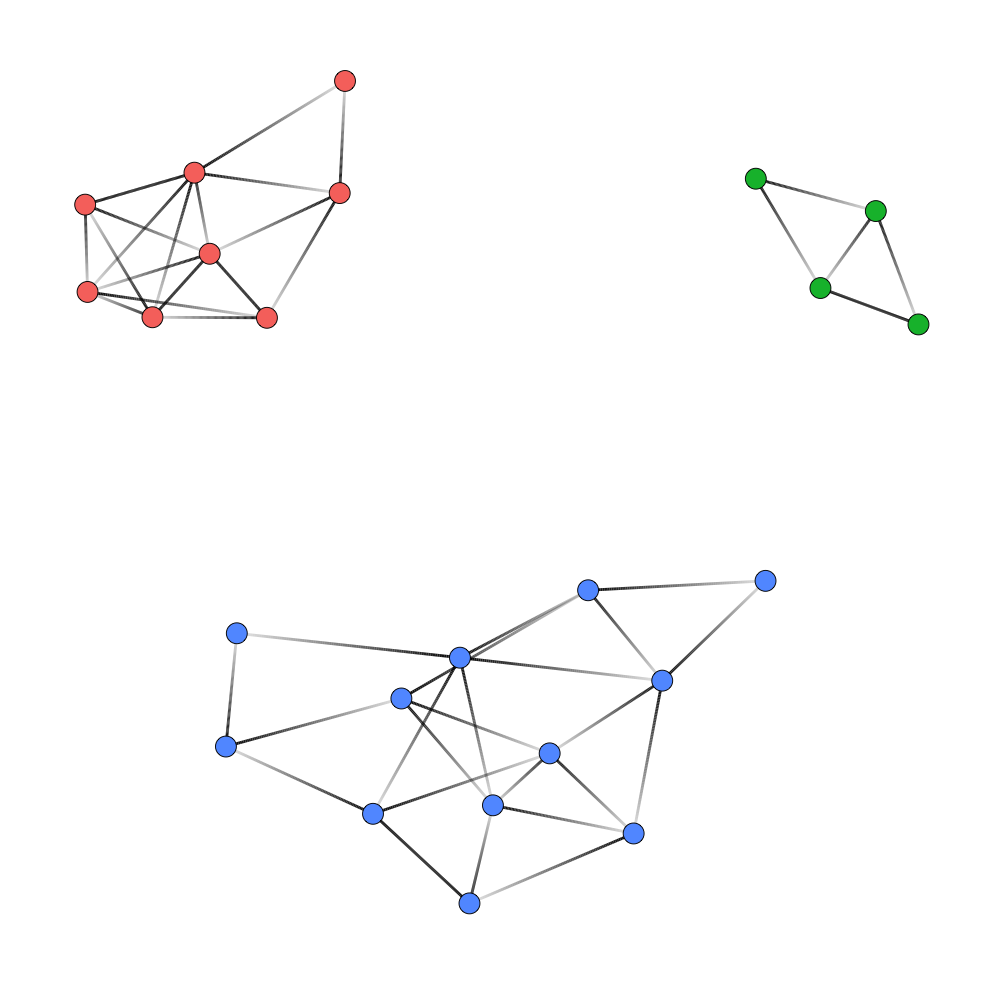
\includegraphics[width = 0.7\textwidth]{Images/struc_zero_nets.png}
\caption[Directed network diagram generated from the example big network adjacency matrix]{Network diagram generated from the example combined network adjacency matrix depicted in Figure \ref{tab:combined}. None of the networks overlap.}
\label{fig:struc_zero_nets}
\end{figure}

\citet{gould1989structures} estimated the statistical significance of their five broker roles using a simple $p_1$ model. Their approach does not account for other possible network effects and tie dependencies that are likely to produce distorted results. Modifications were made to \texttt{MPNet} to allow the statistical significance of the different broker roles to be estimated more accurately. The modified software was used in the second set of model estimations to characterise the three open innovation partnerships in terms of the mix of significant broker roles. Table \ref{tab:ergm_params} lists the model parameters used in this study. Appendix D lists the statistical formulae for these parameters. \medskip

\begin{table}[!htbp]
\centering
\resizebox{\textwidth}{!}{%	
\begin{threeparttable}
\footnotesize
\setlength{\tabcolsep}{6pt}
\renewcommand{\arraystretch}{1}
\caption[Exponential random graph model parameters]{Exponential random graph model parameters used in this study*.}
\label{tab:ergm_params}
\begin{tabular}{lcl}
\toprule
\textbf{Parameter} & \textbf{Graphic} & \textbf{Explanation}  \\ \midrule
\textbf{Purely structural effects} & & \\
Arc (edge) & \begin{minipage}{.2\textwidth} \centering 
\includegraphics[width=0.4\linewidth]{Images/Arc} \end{minipage} & \begin{tabular}[c]{l}Baseline tendency for a tie to form\\ effects.\end{tabular} \\ \\
Reciprocity (mutuality)	& \begin{minipage}{.2\textwidth} \centering 
\includegraphics[width=0.4\linewidth]{Images/Reciprocity} \end{minipage} & \begin{tabular}[c]{l}Tendency for a tie from one actor to a second when there\\ is already a tie from the second to the first.\end{tabular} \\ \\ TwoPath (simple connectivity) & \begin{minipage}{.2\textwidth} \centering 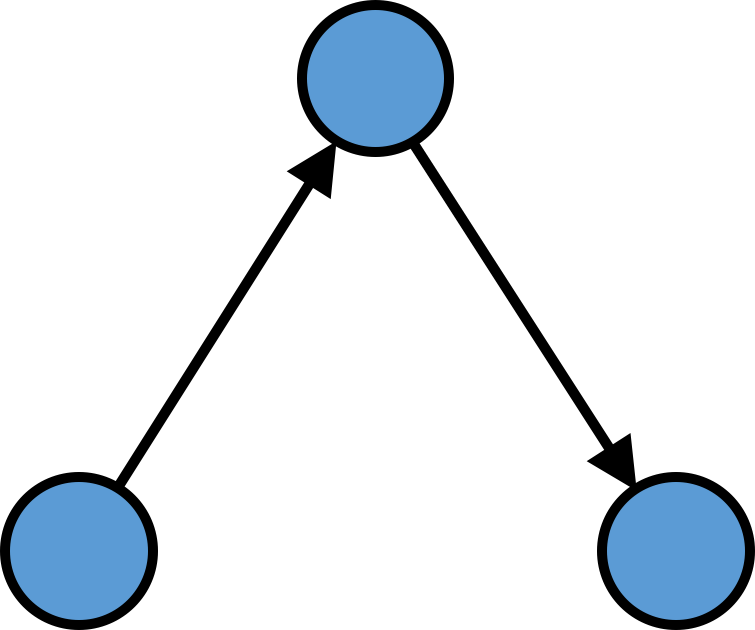
\includegraphics[width=0.4\linewidth]{Images/TwoPath} \end{minipage} & \begin{tabular}[c]{l}Tendency for ties to form as part of simple path formations. \end{tabular} \\ \\
AinS (popularity spread) & \begin{minipage}{.2\textwidth} \centering 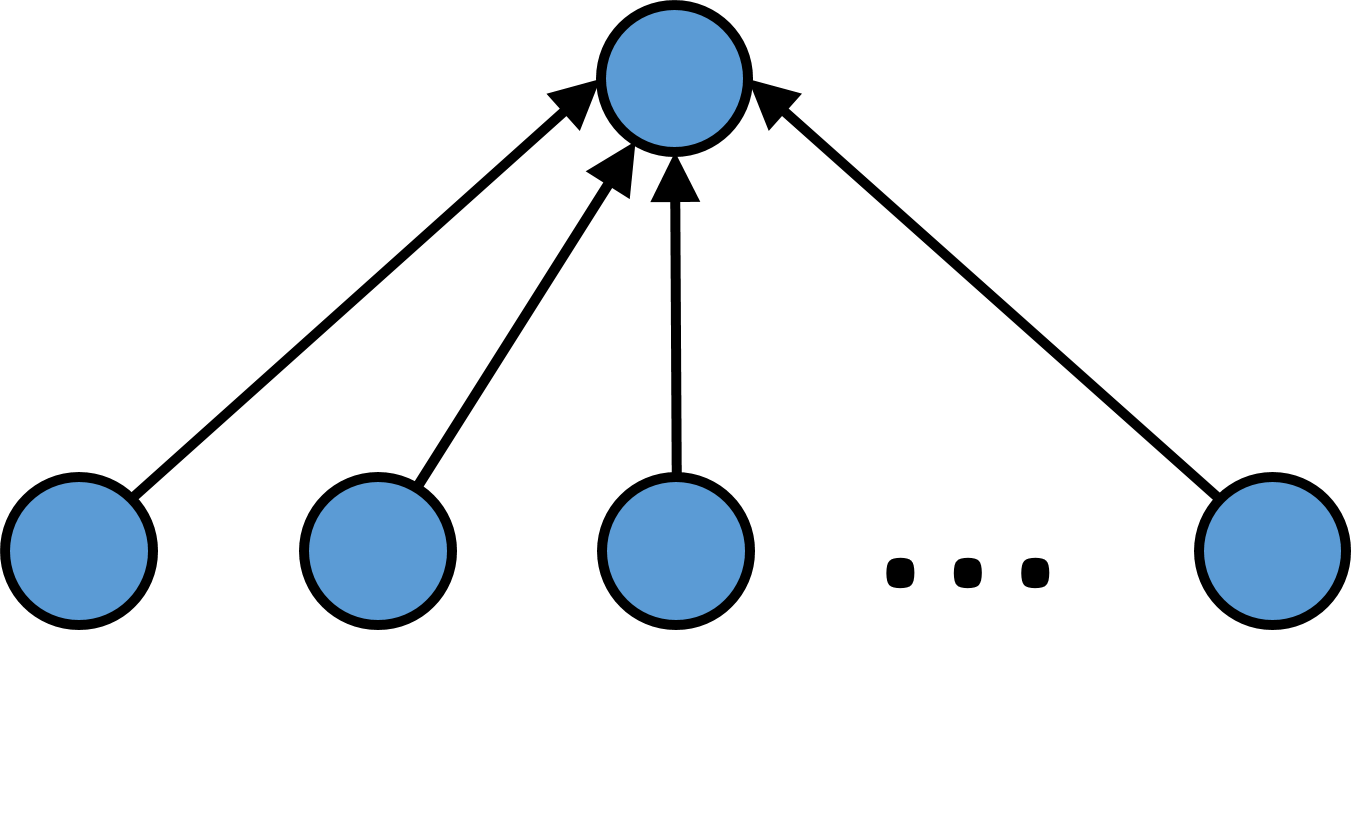
\includegraphics[width=0.6\linewidth]{Images/AinS} \end{minipage} & \begin{tabular}[c]{l}Propensity for dispersion in the in-degree distribution,\\ indicating there are a few highly popular actors. \end{tabular} \\ \\
AoutS (activity spread) & \begin{minipage}{.2\textwidth} \centering 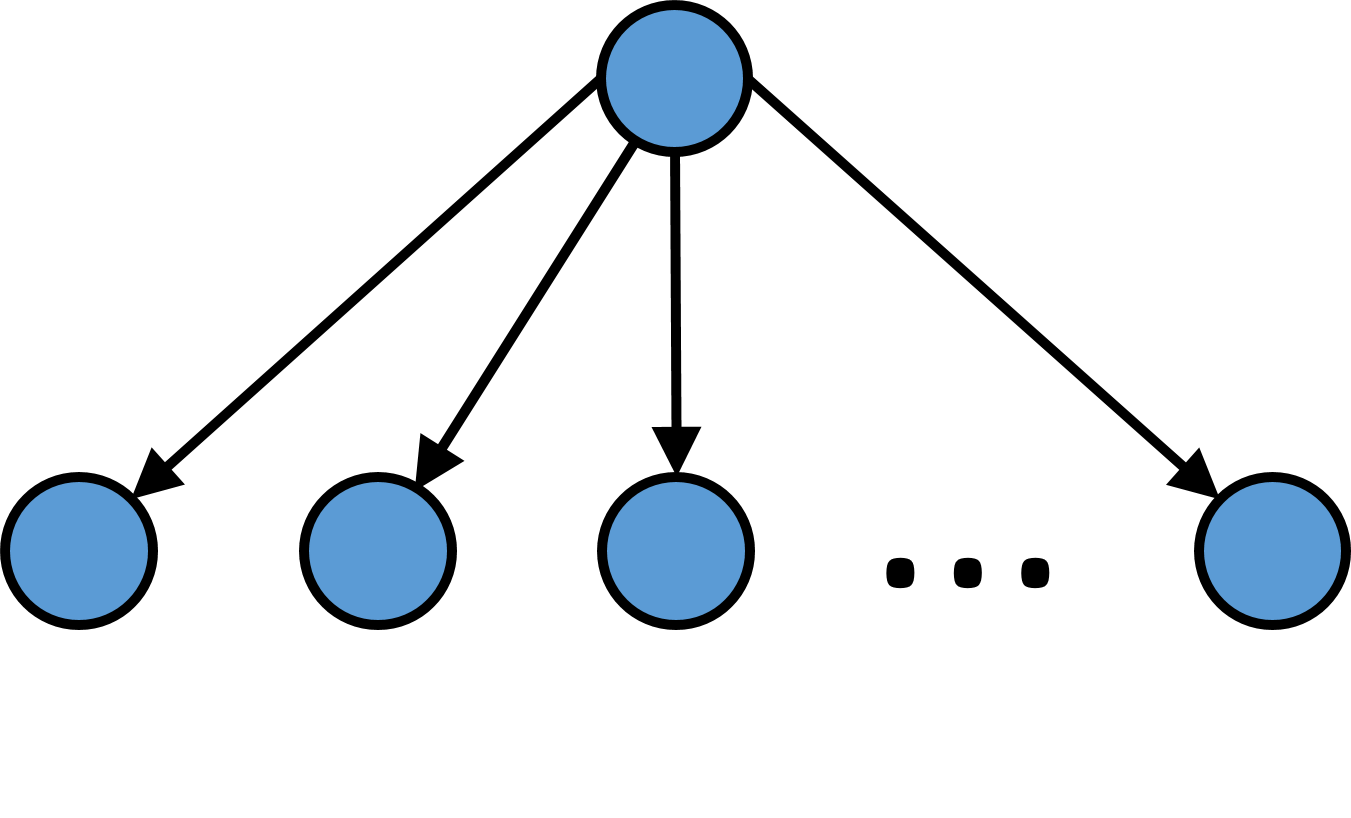
\includegraphics[width=0.6\linewidth]{Images/AoutS} \end{minipage} & \begin{tabular}[c]{l}Propensity for dispersion in the out-degree distribution,\\ indicating there are a few highly active actors. \end{tabular}  \\ \\
AT-T (path closure) & \begin{minipage}{.2\textwidth} \centering 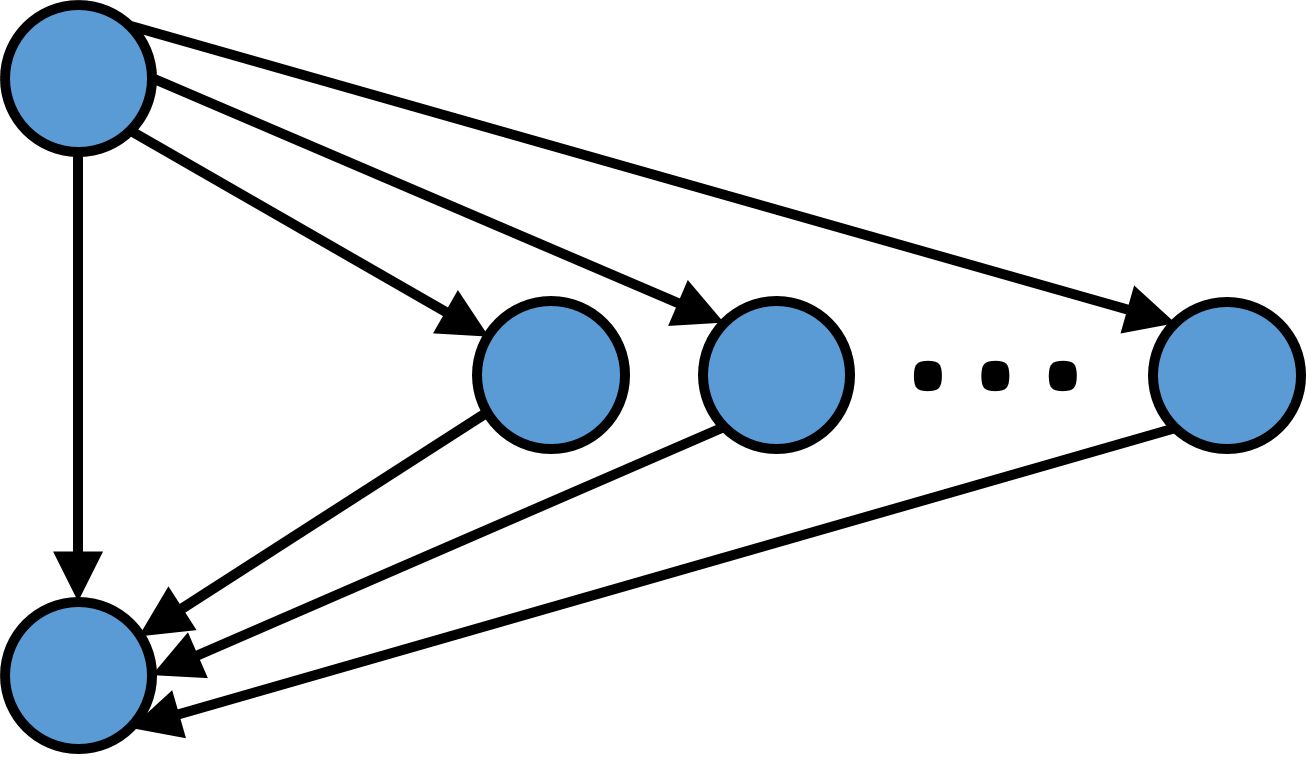
\includegraphics[width=0.6\linewidth]{Images/AT-T} \end{minipage} & \begin{tabular}[c]{l}Propensity for ties to form as part of transitive triad or a\\ multiple transitive configuration. \end{tabular} \\ \\
A2P (multiple connectivity) & \begin{minipage}{.2\textwidth} \centering 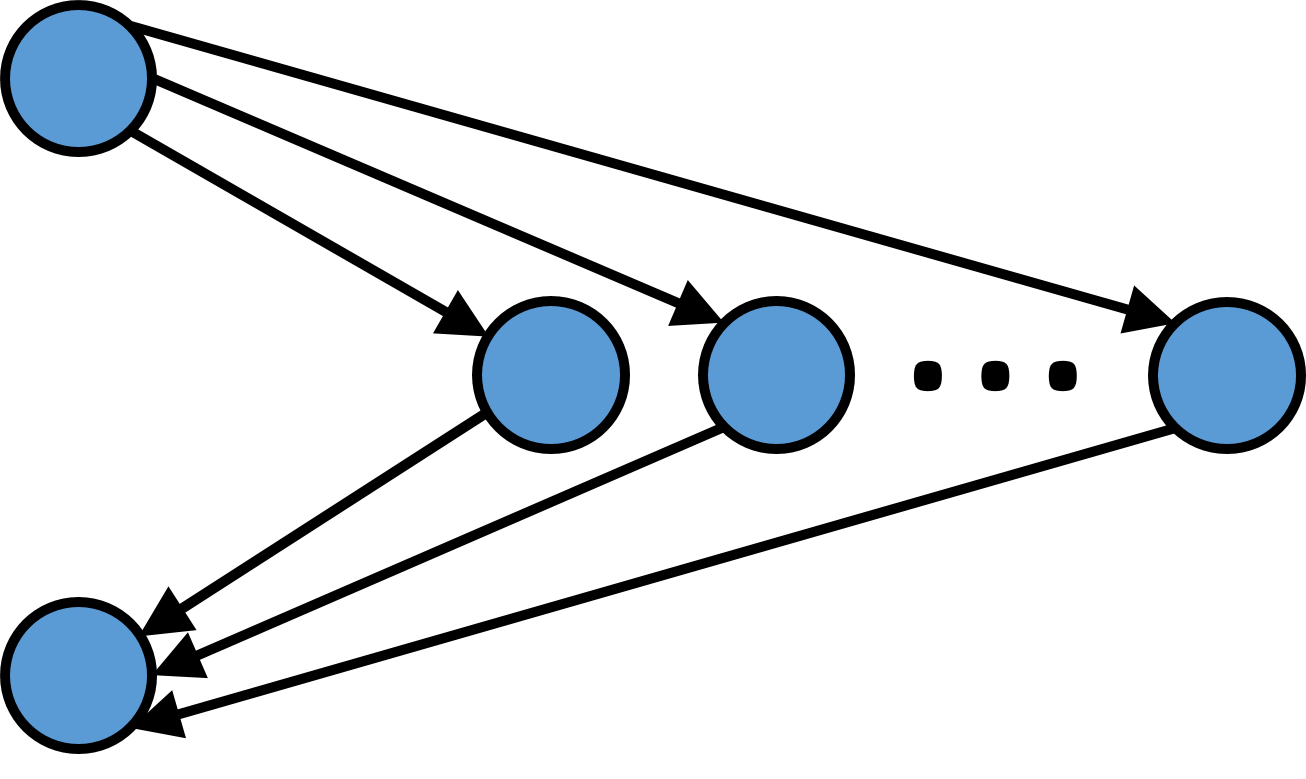
\includegraphics[width=0.6\linewidth]{Images/A2P} \end{minipage} & \begin{tabular}[c]{l}Propensity for ties to form as part of formations involving\\ multiple short paths between actors. \end{tabular} \\ \\
\textbf{Actor-relation effects} & & \\
Attribute sender & \begin{minipage}{.2\textwidth} \centering 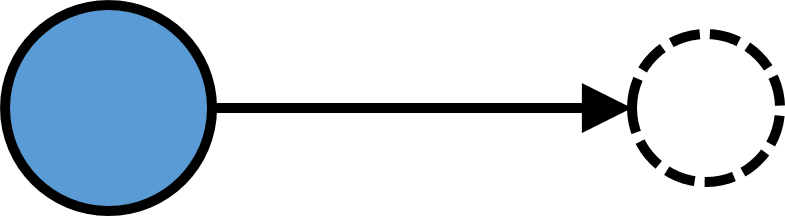
\includegraphics[width=0.4\linewidth]{Images/Sender} \end{minipage}	& \begin{tabular}[c]{l}Propensity for a tie to be directed from an actor with a\\ particular attribute. \end{tabular} \\ \\
Attribute receiver & \begin{minipage}{.2\textwidth} \centering 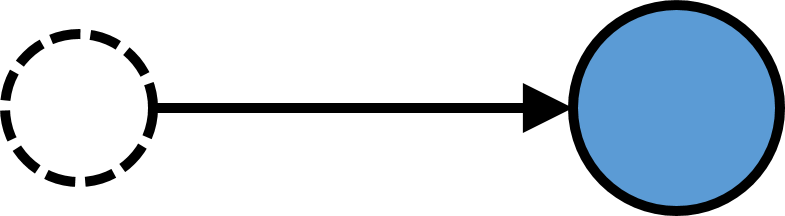
\includegraphics[width=0.4\linewidth]{Images/Receiver} \end{minipage} & \begin{tabular}[c]{l}Propensity for a tie to be directed toward an actor with a\\ particular attribute. \end{tabular} \\ \\
Attribute difference & \begin{minipage}{.2\textwidth} \centering 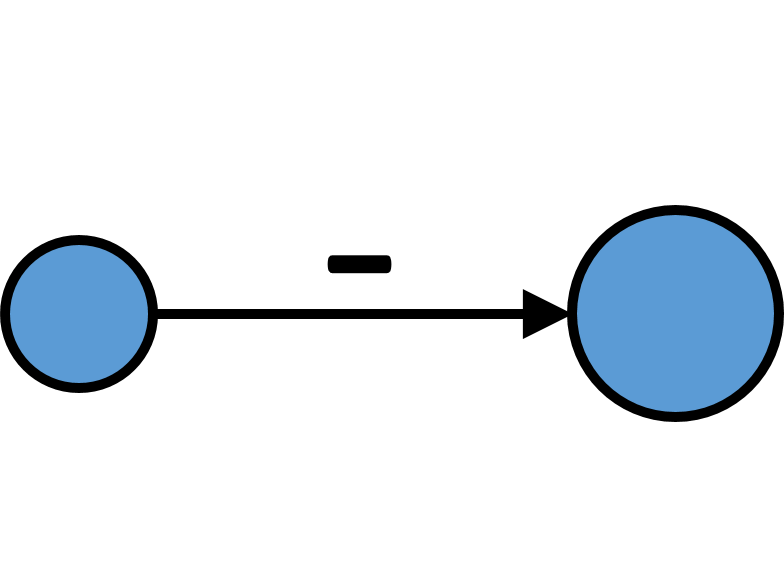
\includegraphics[width=0.4\linewidth]{Images/Difference} \end{minipage} & \begin{tabular}[c]{l}Propensity for a tie to form between actors with a similar\\ continuous attribute. \end{tabular} \\ \\
Attribute match & \begin{minipage}{.2\textwidth} \centering 
\includegraphics[width=0.4\linewidth]{Images/Match} \end{minipage} & \begin{tabular}[c]{l}Propensity for a tie to form between actors with the same\\ categorical attribute.\end{tabular} \\ \\
Attribute mismatch reciprocity & \begin{minipage}{.2\textwidth} \centering 
\includegraphics[width=0.4\linewidth]{Images/MisMatchReciprocity} \end{minipage} & \begin{tabular}[c]{l}Propensity for a tie to form between actors with a\\ non-matching categorical attribute.\end{tabular} \\ \\
\textbf{Actor-brokerage effects} & & \\
b\textsubscript{O} (liaison role) & \begin{minipage}{.2\textwidth} \centering 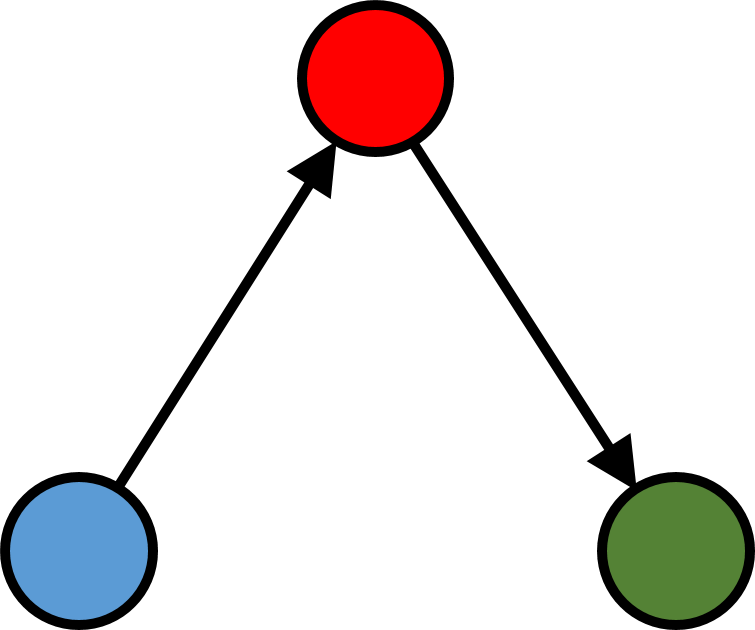
\includegraphics[width=0.4\linewidth]{Images/b_O} \end{minipage} & \begin{tabular}[c]{l}Propensity to have brokers who mediate communication\\ between two individuals from different groups, neither of\\ which they belong to.\end{tabular}\\ \\
b\textsubscript{IO} (representative role) & \begin{minipage}{.2\textwidth} \centering 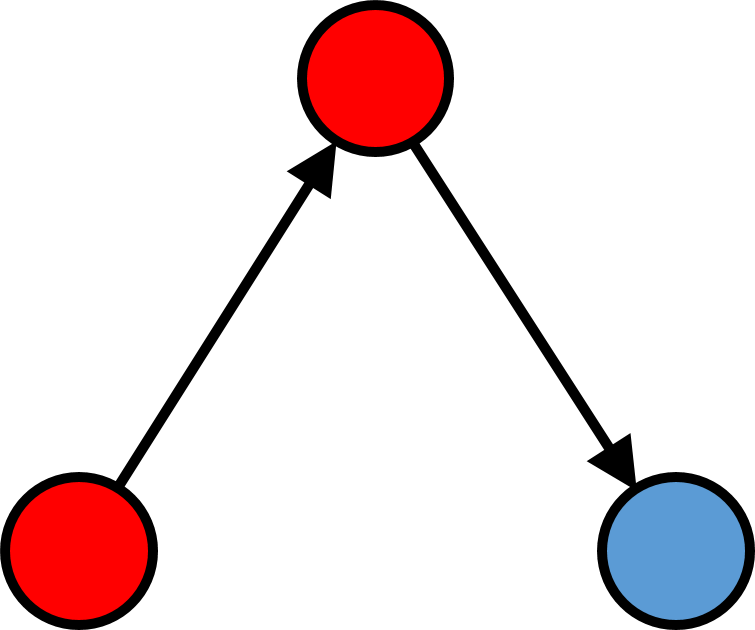
\includegraphics[width=0.4\linewidth]{Images/b_IO} \end{minipage} & \begin{tabular}[c]{l}Propensity to have brokers who mediate communication\\ from in-group members to out-group members. \end{tabular}\\ \\
b\textsubscript{OI} (gatekeeper role) & \begin{minipage}{.2\textwidth} \centering 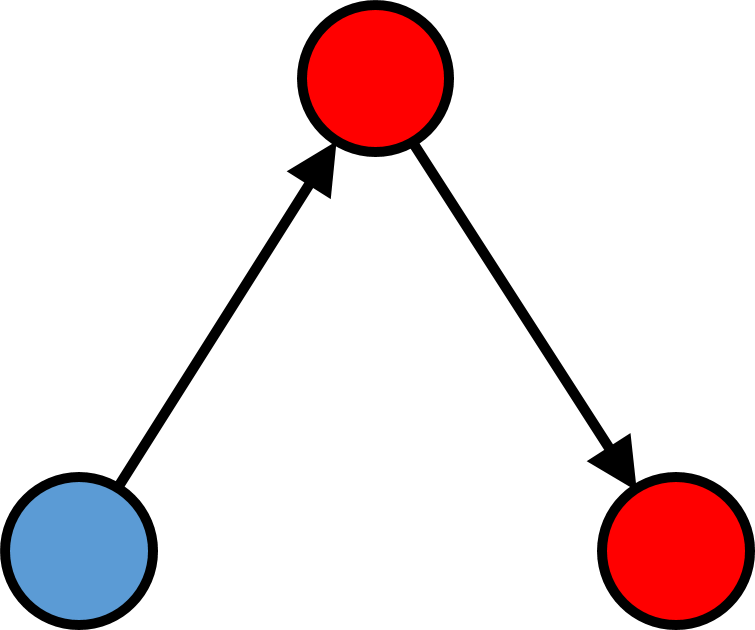
\includegraphics[width=0.4\linewidth]{Images/b_OI} \end{minipage} & \begin{tabular}[c]{l}Propensity to have brokers who mediate communication\\ from out-group members to in-group members. \end{tabular}\\ \\
w\textsubscript{O} (itinerant broker) & \begin{minipage}{.2\textwidth} \centering 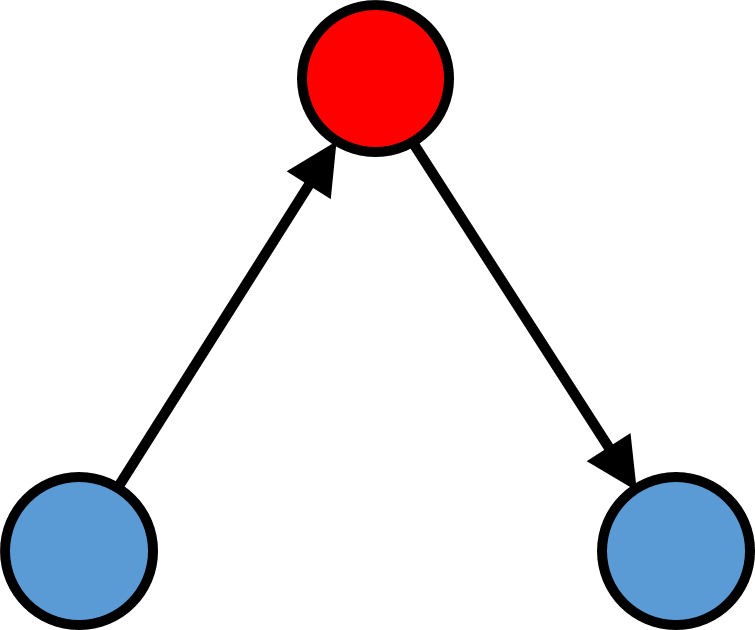
\includegraphics[width=0.4\linewidth]{Images/w_O} \end{minipage} & \begin{tabular}[c]{l}Propensity to have brokers who mediate communication\\ between two individuals from a single group to which they\\ do not belong. \end{tabular}\\ 
w\textsubscript{I} (coordination role) & \begin{minipage}{.2\textwidth} \centering 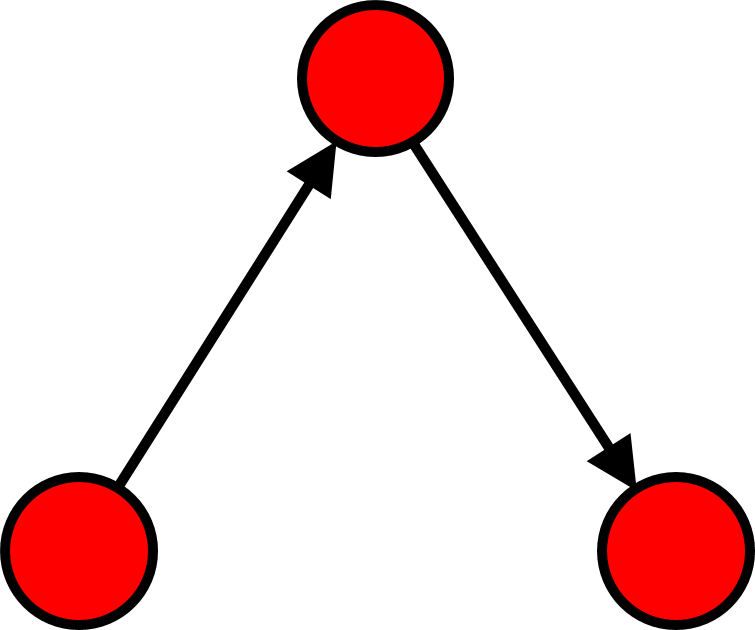
\includegraphics[width=0.4\linewidth]{Images/w_I} \end{minipage} & \begin{tabular}[c]{l}Propensity to have brokers who mediate communication\\ between two individuals from his or her own group. \end{tabular}\\ \\	
\textbf{Network covariate effects} & & \\
Dyadic covariate & \begin{minipage}{.2\textwidth} \centering 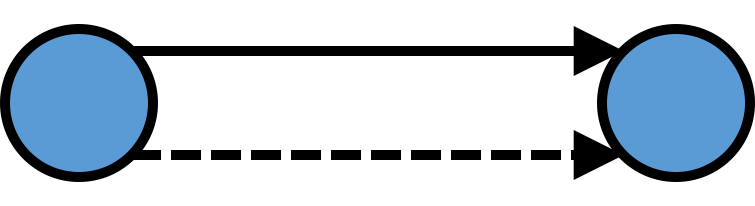
\includegraphics[width=0.4\linewidth]{Images/DyadicCovariate} \end{minipage} & \begin{tabular}[c]{l}Propensity for a tie of one type to form from one actor to\\ another if a tie of another type is already present, though\\ the covariate network is fixed (i.e. exogenous) in the\\ model, and so cannot vary. \end{tabular} \\\bottomrule
\end{tabular}

\begin{tablenotes}
\footnotesize
* Refer to Appendix D for each parameter's network statistic.
\end{tablenotes}

\end{threeparttable}
%
}
\end{table}

\section{Qualitative procedures}

\subsection{Data collection}

Follow-up interviews with a subset of survey participants make up the qualitative component of this study. Results from the exploratory data analysis of survey data was used to identify potential interviewees. Two criteria were used to identify which participants to interview, namely their network position and availability or willingness to be interviewed. Network position refers to the centrality of actors in the [tacit + explicit] knowledge provider network. The aim was to identify central and peripheral actors in the network, i.e. both powerful and less powerful actors. Some of the more central participants were unavailable to be interviewed because of pressing work commitments. Others were not comfortable being interviewed in English. 

\subsubsection{Semi-structured interview questions}

The semi-structured interview questions were designed to explore the following constructs: industry context, partner history, the chronology of key events, the strength of the partnership, organisational culture, power relations, attitudes towards knowledge sharing and innovation, levels of motivation and trust, governance structures, and organisational learning capacity. Refer to Table \ref{tab:interview} in Appendix C for the list of questions used in the interviews. Interviews were designed to be completed in under an hour. The administration of semi-structured interviews was subject to ethics approval. 

\subsubsection{Interview protocol}

All the interviews were done by the author, either face-to-face or via video conference (using Skype\texttrademark). Each interview was recorded (using a digital memo recorder in the case of face-to-face interviews and a third-party plug-in recorder for Skype\texttrademark\ interviews). At the beginning of each interview, participants were asked to sign a consent form, permitting the use of the interview transcript in this study. Only then could recording start. Before each interview, participants had the opportunity to discuss their psychological profile based on their online survey responses. This was done for two reasons. Firstly, to make interviewees feel comfortable, and secondly, to check if their responses to the online survey made any sense. \medskip

The number of questions asked in each interview varied according to the individual circumstances. Some interviewees were not well-placed to comment on event chronology, partner history, or formal governance mechanisms. Consequently, some questions were skipped over. Each interviewee was asked to comment on network diagrams depicting knowledge sharing, idea generation, and trust relations in their specific open innovation partnership. Showing network diagrams helped maintain a strong focus on partner behaviour and to solicit useful contextual information. \medskip

After each interview, interviewees were thanked and told they would receive via email a copy of the transcribed interview. They could withdraw their consent for the use of transcribed data if they felt uncomfortable with the contents thereof. 

\subsection{Data processing}

\subsubsection{Transcription of audio recordings}

The audio recordings of each interview were saved as MP3 files. Unfortunately, one Skype\texttrademark\ interview could not be transcribed as it failed to record correctly. The audio quality of another Skype\texttrademark\ recording was too poor for accurate transcription. Usable audio files were uploaded to a third-party transcription service (\url{http://www.transcriberonline.com/}). This service used manual transcribing that yielded very accurate transcriptions. The turnaround time for completing audio transcriptions was around three days. Transcriptions were provided as a Microsoft Word\texttrademark\ documents. Each interviewee was allowed to comment on their interview transcription before qualitative analysis. None of the interviewees reported any issues. 

\subsubsection{Qualitative data analysis software}

Transcriptions were analysed using NVivo\texttrademark, a qualitative data analysis software (QDAS) package. This package facilitates manual coding of qualitative data and subsequent organisation and analysis of coded data \citep{bazeley2013qualitative}. NVivo\texttrademark\ allows one to work directly with the text, selecting passages, and doing coding onscreen. The same passage of text can have multiple codes. It is easy to insert annotations, comments, or analytic memos related to a specific code. Not only is it possible to immediately review coded text, one can easily combine, assemble, and re-arrange codes into new categories or themes in the process of \enquote{coding\hyp{}on} \citep{richards2012readme}. NVivo\texttrademark\ supports complex data queries, offers different ways to visualise coded data, and provides various analytical reports \citep{bazeley2013qualitative}. 

\subsubsection{Critical realist analytical framework} \label{sss:cr_framewk}

A code in qualitative data analysis is usually a word or short phrase that captures a meaningful attribute for a portion of text-based or visual data \citep{saldana2015coding}. There are many ways to code, but all share a common goal, namely extracting meaning from messy and unstructured qualitative data \citep{richards2012readme}. The process of coding involves assigning labels to individual words or chunks of text, sorting labels into different categories, grouping categories into broad themes, and then figuring out what these themes reveal about a given context. \medskip

Unfortunately, the literature on how to code qualitative data from a critical realist perspective is quite scant \citep{fletcher2017applying}. A key objective in critical realism is to look for patterns in empirical data that contribute to the generation of broad propositions or specific hypotheses about causal mechanisms \citep{zachariadis2013methodological}. This study uses a critical realist analytical framework developed by \cite{bygstad2016identifying} and further refined by \citet{mcavoy2018critical}. Figure \ref{fig:cr_steps} outlines the three main steps of this analytical framework. \medskip
 
\begin{figure}
\centering
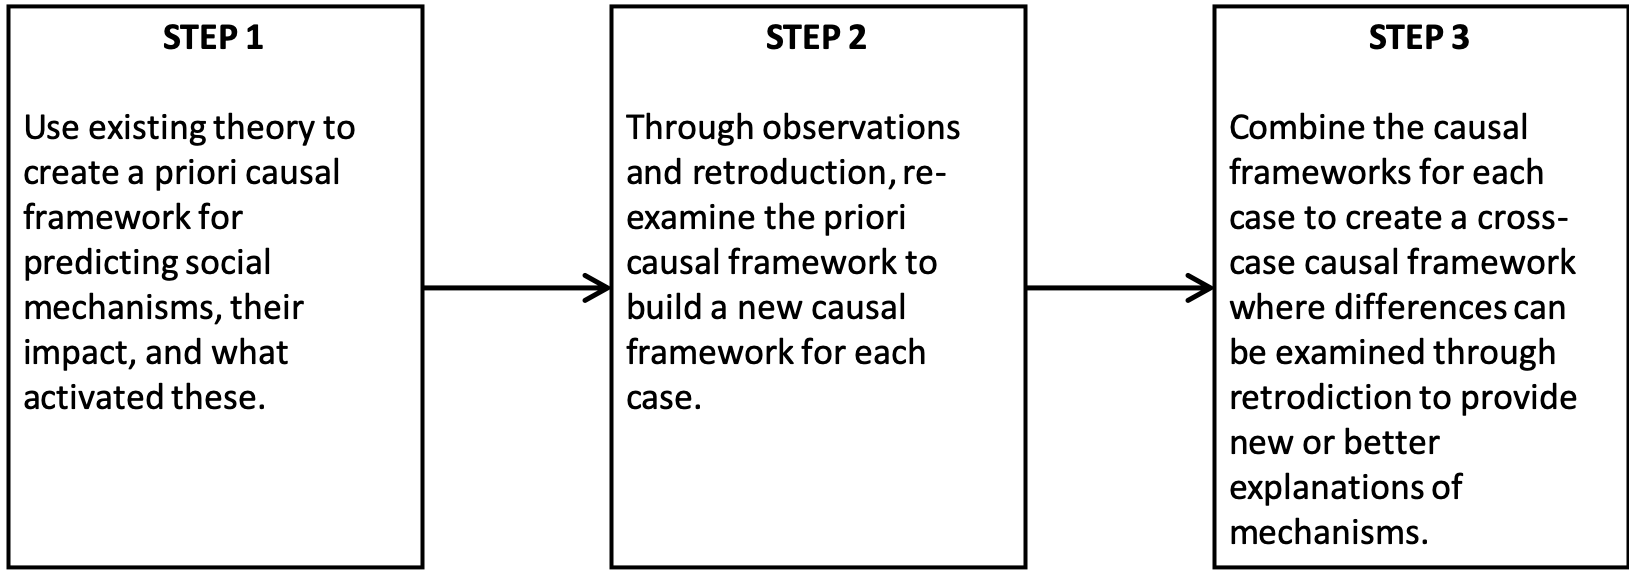
\includegraphics[width = 0.9\textwidth,
height = 0.7\textheight, keepaspectratio]{Images/cr_steps.png}
\caption[Critical realist analytical process]{Critical realist analytical process (after \cite{mcavoy2018critical})}
\label{fig:cr_steps}
\end{figure}

This study argues that agency lies at the heart of tacit knowledge sharing. It embraces \citet{parsons1937structure}'s idea that individuals act to satisfy innate needs and that existing conditions and available means moderate their actions \citep{loyal2001agency}. The first step of our critical realist approach assumes that individuals choose to share or seek out tacit knowledge to satisfy an innate need for self-determination and adhere to subjective norms. Tempering the decision to share or seek tacit knowledge are external factors such as the presence of boundaries (e.g. organisational, disciplinary, or cultural boundaries), rules of engagement (e.g. contractual arrangements, appropriability regimes), trust (i.e. interpersonal and inter-organisational trust), and power relations (e.g.power-over versus power-to). We argue that skilled brokerage plays a crucial role in helping individuals overcome boundaries, build trust, and manage power relations. Figure \ref{fig:agency_structure} represents the prior causal framework based on \citet{loyal2001agency}'s refinement of \citet{parsons1937structure}'s idea. We use the theories of self-determination \citep{ryan2000self}, planned behaviour \citep{ajzen1985intentions}, social exchange \citep{blau1964exchange}, power-relations \citep{emerson1962power}, and brokerage \citep{marsden1982brokerage,burt2005brokerage,obstfeld2014brokerage} to elaborate the framework through a set of propositions, which serve as a starting point for our critical realist analysis (the first step of analysis). \medskip

The second step combines the results of the social network analysis with the coding of semi-structured interviews. We derived a set of provisional codes from the theoretical propositions developed in Chapters 2 and 3. The provisional codes were expanded upon through inductive coding of interview transcripts. Expanded codes were then grouped into category codes. Coded segments of interview transcripts describe the initial constructs in context, draw attention to hidden constructs, and provide a foundation for inductively forming higher-level categories of codes \citep{saldana2015coding}. Efforts to discover unobserved mechanisms and interacting structures also help expose potential researcher bias with initial constructs. \medskip

In the final third step, we use the logic of retroduction to develop a causal framework for each case and then the logic of retrodiction to combine the causal frameworks for each case, allowing us to provide new or better explanations of tacit knowledge sharing mechanisms \citep{mcavoy2018critical}. We end up with an updated set of propositions that can account for what is happening in practice and what is driving practice. Figure \ref{fig:coding_process} summarises the critical realist process used in this study. Codes from each case were recorded into a universal codebook (a codebook is a compilation of all the codes, their content descriptions, and a brief data example for reference) \citep{guest2011applied}. 

% point to appendix.

\begin{sidewaysfigure}
\centering
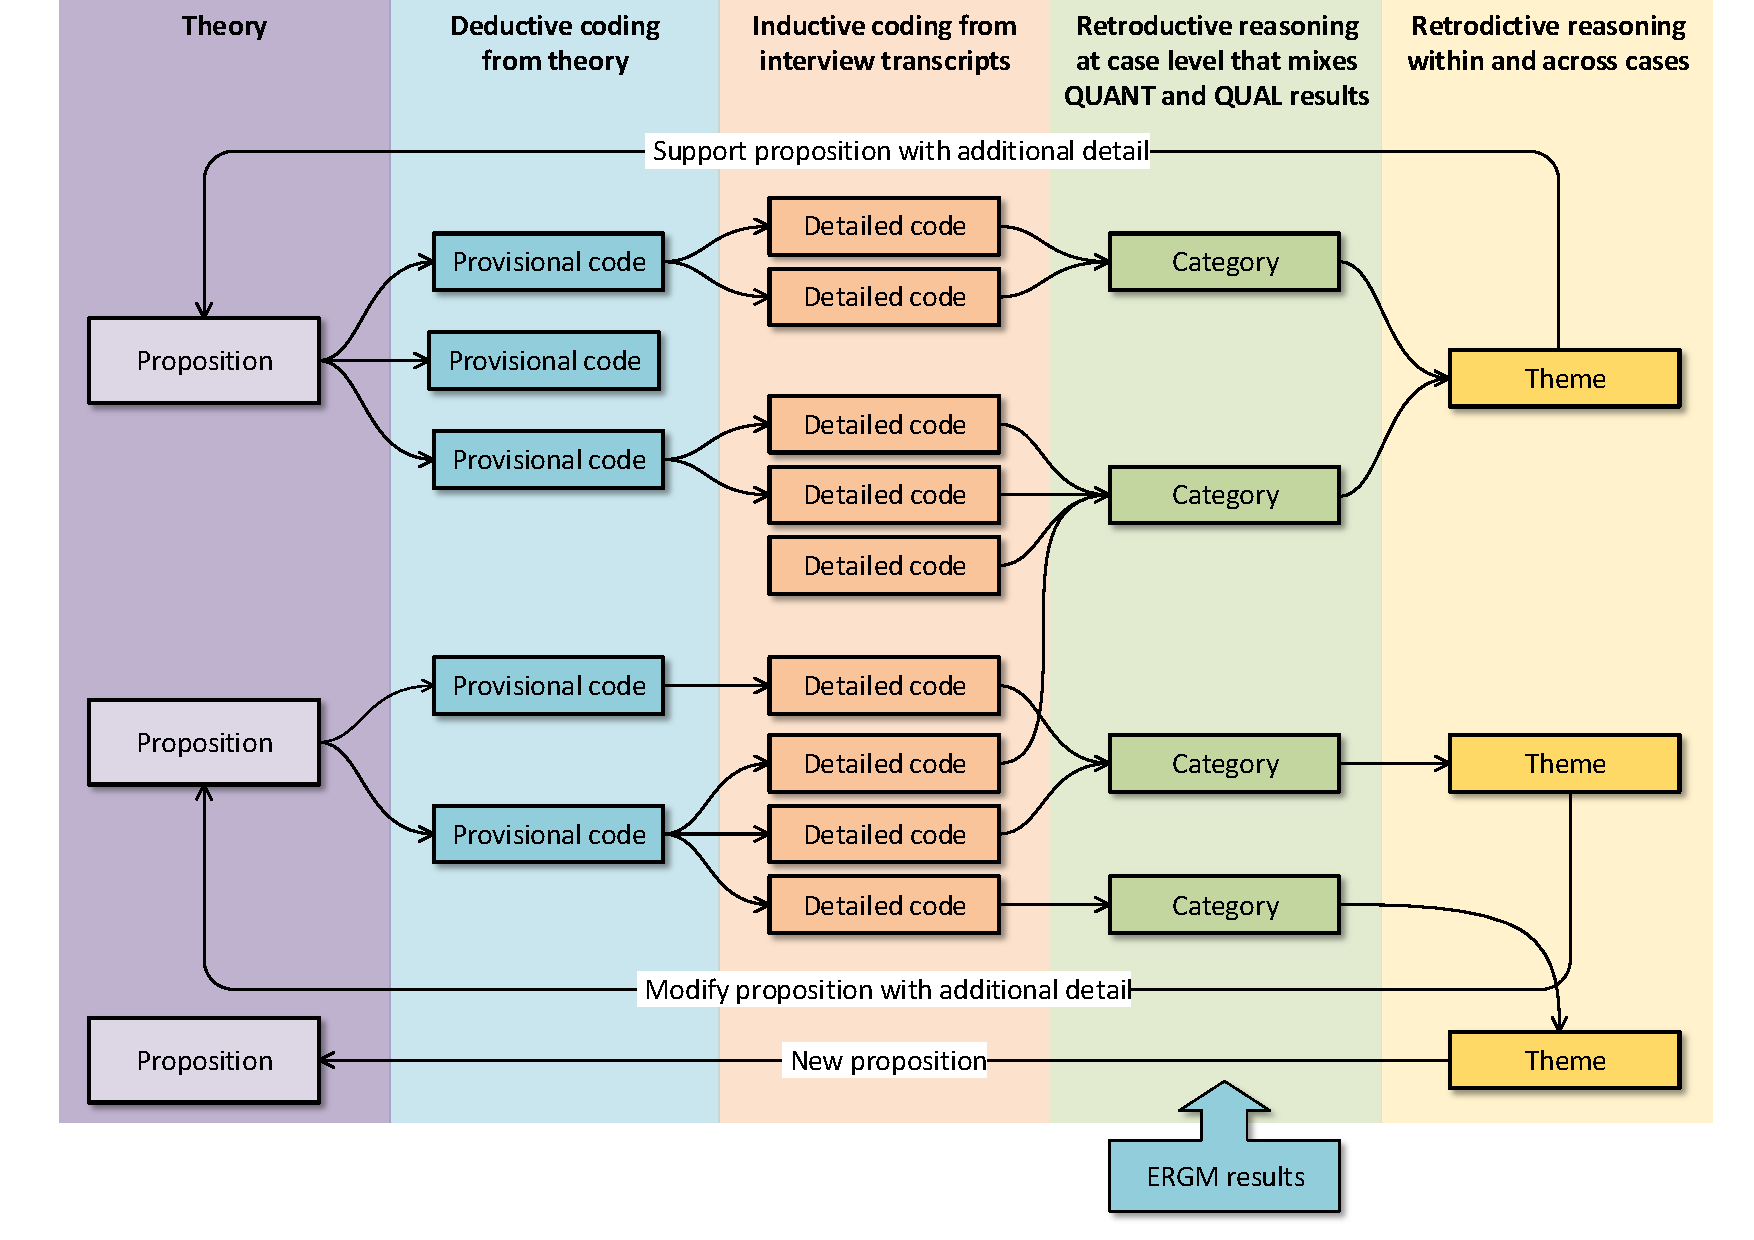
\includegraphics[width = 0.9\textwidth,
height = 0.7\textheight, keepaspectratio]{Images/CR.pdf}
\caption[Critical realist coding process]{Critical realist coding process.}
\label{fig:coding_process}
\end{sidewaysfigure}

\section{Summary}

This thesis employs a mixed-methods approach to examine the social mechanisms that shape tacit knowledge sharing in three open innovation partnerships. An online survey was used to gather data about individual participants in each partnership and their social relations with fellow participants. Survey data were analysed using a combination of descriptive and statistical social network analysis techniques. The descriptive analysis measured actor centrality and two-path brokerage whereas the statistical analysis used ERGMs to assess the relative abundance or absence of specific network configurations. Semi-structured interviews involving a subset of the survey participants complemented the social network analysis. Mixing quantitative network and qualitative interview data can be fraught due to the complex ontological and epistemological issues involved. For this reason, a critical realist perspective was used to interpret quantitative and qualitative results. This thesis breaks new ground in applying a critical realist approach to mixed-method social network analysis. \medskip

The next chapter details the innovation challenge in each of the three open innovation cases recruited. Each case is quite different looking at their industrial context, the stage they are at, participant numbers, their demographic features, spatial proximity to one another, and patterns of social interaction. 